\documentclass[11pt]{article}

    \usepackage[breakable]{tcolorbox}
    \usepackage{parskip} % Stop auto-indenting (to mimic markdown behaviour)
    

    % Basic figure setup, for now with no caption control since it's done
    % automatically by Pandoc (which extracts ![](path) syntax from Markdown).
    \usepackage{graphicx}
    % Maintain compatibility with old templates. Remove in nbconvert 6.0
    \let\Oldincludegraphics\includegraphics
    % Ensure that by default, figures have no caption (until we provide a
    % proper Figure object with a Caption API and a way to capture that
    % in the conversion process - todo).
    \usepackage{caption}
    \DeclareCaptionFormat{nocaption}{}
    \captionsetup{format=nocaption,aboveskip=0pt,belowskip=0pt}

    \usepackage{float}
    \floatplacement{figure}{H} % forces figures to be placed at the correct location
    \usepackage{xcolor} % Allow colors to be defined
    \usepackage{enumerate} % Needed for markdown enumerations to work
    \usepackage{geometry} % Used to adjust the document margins
    \usepackage{amsmath} % Equations
    \usepackage{amssymb} % Equations
    \usepackage{textcomp} % defines textquotesingle
    % Hack from http://tex.stackexchange.com/a/47451/13684:
    \AtBeginDocument{%
        \def\PYZsq{\textquotesingle}% Upright quotes in Pygmentized code
    }
    \usepackage{upquote} % Upright quotes for verbatim code
    \usepackage{eurosym} % defines \euro

    \usepackage{iftex}
    \ifPDFTeX
        \usepackage[T1]{fontenc}
        \IfFileExists{alphabeta.sty}{
              \usepackage{alphabeta}
          }{
              \usepackage[mathletters]{ucs}
              \usepackage[utf8x]{inputenc}
          }
    \else
        \usepackage{fontspec}
        \usepackage{unicode-math}
    \fi

    \usepackage{fancyvrb} % verbatim replacement that allows latex
    \usepackage{grffile} % extends the file name processing of package graphics
                         % to support a larger range
    \makeatletter % fix for old versions of grffile with XeLaTeX
    \@ifpackagelater{grffile}{2019/11/01}
    {
      % Do nothing on new versions
    }
    {
      \def\Gread@@xetex#1{%
        \IfFileExists{"\Gin@base".bb}%
        {\Gread@eps{\Gin@base.bb}}%
        {\Gread@@xetex@aux#1}%
      }
    }
    \makeatother
    \usepackage[Export]{adjustbox} % Used to constrain images to a maximum size
    \adjustboxset{max size={0.9\linewidth}{0.9\paperheight}}

    % The hyperref package gives us a pdf with properly built
    % internal navigation ('pdf bookmarks' for the table of contents,
    % internal cross-reference links, web links for URLs, etc.)
    \usepackage{hyperref}
    % The default LaTeX title has an obnoxious amount of whitespace. By default,
    % titling removes some of it. It also provides customization options.
    \usepackage{titling}
    \usepackage{longtable} % longtable support required by pandoc >1.10
    \usepackage{booktabs}  % table support for pandoc > 1.12.2
    \usepackage{array}     % table support for pandoc >= 2.11.3
    \usepackage{calc}      % table minipage width calculation for pandoc >= 2.11.1
    \usepackage[inline]{enumitem} % IRkernel/repr support (it uses the enumerate* environment)
    \usepackage[normalem]{ulem} % ulem is needed to support strikethroughs (\sout)
                                % normalem makes italics be italics, not underlines
    \usepackage{soul}      % strikethrough (\st) support for pandoc >= 3.0.0
    \usepackage{mathrsfs}
    

    
    % Colors for the hyperref package
    \definecolor{urlcolor}{rgb}{0,.145,.698}
    \definecolor{linkcolor}{rgb}{.71,0.21,0.01}
    \definecolor{citecolor}{rgb}{.12,.54,.11}

    % ANSI colors
    \definecolor{ansi-black}{HTML}{3E424D}
    \definecolor{ansi-black-intense}{HTML}{282C36}
    \definecolor{ansi-red}{HTML}{E75C58}
    \definecolor{ansi-red-intense}{HTML}{B22B31}
    \definecolor{ansi-green}{HTML}{00A250}
    \definecolor{ansi-green-intense}{HTML}{007427}
    \definecolor{ansi-yellow}{HTML}{DDB62B}
    \definecolor{ansi-yellow-intense}{HTML}{B27D12}
    \definecolor{ansi-blue}{HTML}{208FFB}
    \definecolor{ansi-blue-intense}{HTML}{0065CA}
    \definecolor{ansi-magenta}{HTML}{D160C4}
    \definecolor{ansi-magenta-intense}{HTML}{A03196}
    \definecolor{ansi-cyan}{HTML}{60C6C8}
    \definecolor{ansi-cyan-intense}{HTML}{258F8F}
    \definecolor{ansi-white}{HTML}{C5C1B4}
    \definecolor{ansi-white-intense}{HTML}{A1A6B2}
    \definecolor{ansi-default-inverse-fg}{HTML}{FFFFFF}
    \definecolor{ansi-default-inverse-bg}{HTML}{000000}

    % common color for the border for error outputs.
    \definecolor{outerrorbackground}{HTML}{FFDFDF}

    % commands and environments needed by pandoc snippets
    % extracted from the output of `pandoc -s`
    \providecommand{\tightlist}{%
      \setlength{\itemsep}{0pt}\setlength{\parskip}{0pt}}
    \DefineVerbatimEnvironment{Highlighting}{Verbatim}{commandchars=\\\{\}}
    % Add ',fontsize=\small' for more characters per line
    \newenvironment{Shaded}{}{}
    \newcommand{\KeywordTok}[1]{\textcolor[rgb]{0.00,0.44,0.13}{\textbf{{#1}}}}
    \newcommand{\DataTypeTok}[1]{\textcolor[rgb]{0.56,0.13,0.00}{{#1}}}
    \newcommand{\DecValTok}[1]{\textcolor[rgb]{0.25,0.63,0.44}{{#1}}}
    \newcommand{\BaseNTok}[1]{\textcolor[rgb]{0.25,0.63,0.44}{{#1}}}
    \newcommand{\FloatTok}[1]{\textcolor[rgb]{0.25,0.63,0.44}{{#1}}}
    \newcommand{\CharTok}[1]{\textcolor[rgb]{0.25,0.44,0.63}{{#1}}}
    \newcommand{\StringTok}[1]{\textcolor[rgb]{0.25,0.44,0.63}{{#1}}}
    \newcommand{\CommentTok}[1]{\textcolor[rgb]{0.38,0.63,0.69}{\textit{{#1}}}}
    \newcommand{\OtherTok}[1]{\textcolor[rgb]{0.00,0.44,0.13}{{#1}}}
    \newcommand{\AlertTok}[1]{\textcolor[rgb]{1.00,0.00,0.00}{\textbf{{#1}}}}
    \newcommand{\FunctionTok}[1]{\textcolor[rgb]{0.02,0.16,0.49}{{#1}}}
    \newcommand{\RegionMarkerTok}[1]{{#1}}
    \newcommand{\ErrorTok}[1]{\textcolor[rgb]{1.00,0.00,0.00}{\textbf{{#1}}}}
    \newcommand{\NormalTok}[1]{{#1}}

    % Additional commands for more recent versions of Pandoc
    \newcommand{\ConstantTok}[1]{\textcolor[rgb]{0.53,0.00,0.00}{{#1}}}
    \newcommand{\SpecialCharTok}[1]{\textcolor[rgb]{0.25,0.44,0.63}{{#1}}}
    \newcommand{\VerbatimStringTok}[1]{\textcolor[rgb]{0.25,0.44,0.63}{{#1}}}
    \newcommand{\SpecialStringTok}[1]{\textcolor[rgb]{0.73,0.40,0.53}{{#1}}}
    \newcommand{\ImportTok}[1]{{#1}}
    \newcommand{\DocumentationTok}[1]{\textcolor[rgb]{0.73,0.13,0.13}{\textit{{#1}}}}
    \newcommand{\AnnotationTok}[1]{\textcolor[rgb]{0.38,0.63,0.69}{\textbf{\textit{{#1}}}}}
    \newcommand{\CommentVarTok}[1]{\textcolor[rgb]{0.38,0.63,0.69}{\textbf{\textit{{#1}}}}}
    \newcommand{\VariableTok}[1]{\textcolor[rgb]{0.10,0.09,0.49}{{#1}}}
    \newcommand{\ControlFlowTok}[1]{\textcolor[rgb]{0.00,0.44,0.13}{\textbf{{#1}}}}
    \newcommand{\OperatorTok}[1]{\textcolor[rgb]{0.40,0.40,0.40}{{#1}}}
    \newcommand{\BuiltInTok}[1]{{#1}}
    \newcommand{\ExtensionTok}[1]{{#1}}
    \newcommand{\PreprocessorTok}[1]{\textcolor[rgb]{0.74,0.48,0.00}{{#1}}}
    \newcommand{\AttributeTok}[1]{\textcolor[rgb]{0.49,0.56,0.16}{{#1}}}
    \newcommand{\InformationTok}[1]{\textcolor[rgb]{0.38,0.63,0.69}{\textbf{\textit{{#1}}}}}
    \newcommand{\WarningTok}[1]{\textcolor[rgb]{0.38,0.63,0.69}{\textbf{\textit{{#1}}}}}


    % Define a nice break command that doesn't care if a line doesn't already
    % exist.
    \def\br{\hspace*{\fill} \\* }
    % Math Jax compatibility definitions
    \def\gt{>}
    \def\lt{<}
    \let\Oldtex\TeX
    \let\Oldlatex\LaTeX
    \renewcommand{\TeX}{\textrm{\Oldtex}}
    \renewcommand{\LaTeX}{\textrm{\Oldlatex}}
    % Document parameters
    % Document title
    \title{lab5}
    
    
    
    
    
    
    
% Pygments definitions
\makeatletter
\def\PY@reset{\let\PY@it=\relax \let\PY@bf=\relax%
    \let\PY@ul=\relax \let\PY@tc=\relax%
    \let\PY@bc=\relax \let\PY@ff=\relax}
\def\PY@tok#1{\csname PY@tok@#1\endcsname}
\def\PY@toks#1+{\ifx\relax#1\empty\else%
    \PY@tok{#1}\expandafter\PY@toks\fi}
\def\PY@do#1{\PY@bc{\PY@tc{\PY@ul{%
    \PY@it{\PY@bf{\PY@ff{#1}}}}}}}
\def\PY#1#2{\PY@reset\PY@toks#1+\relax+\PY@do{#2}}

\@namedef{PY@tok@w}{\def\PY@tc##1{\textcolor[rgb]{0.73,0.73,0.73}{##1}}}
\@namedef{PY@tok@c}{\let\PY@it=\textit\def\PY@tc##1{\textcolor[rgb]{0.24,0.48,0.48}{##1}}}
\@namedef{PY@tok@cp}{\def\PY@tc##1{\textcolor[rgb]{0.61,0.40,0.00}{##1}}}
\@namedef{PY@tok@k}{\let\PY@bf=\textbf\def\PY@tc##1{\textcolor[rgb]{0.00,0.50,0.00}{##1}}}
\@namedef{PY@tok@kp}{\def\PY@tc##1{\textcolor[rgb]{0.00,0.50,0.00}{##1}}}
\@namedef{PY@tok@kt}{\def\PY@tc##1{\textcolor[rgb]{0.69,0.00,0.25}{##1}}}
\@namedef{PY@tok@o}{\def\PY@tc##1{\textcolor[rgb]{0.40,0.40,0.40}{##1}}}
\@namedef{PY@tok@ow}{\let\PY@bf=\textbf\def\PY@tc##1{\textcolor[rgb]{0.67,0.13,1.00}{##1}}}
\@namedef{PY@tok@nb}{\def\PY@tc##1{\textcolor[rgb]{0.00,0.50,0.00}{##1}}}
\@namedef{PY@tok@nf}{\def\PY@tc##1{\textcolor[rgb]{0.00,0.00,1.00}{##1}}}
\@namedef{PY@tok@nc}{\let\PY@bf=\textbf\def\PY@tc##1{\textcolor[rgb]{0.00,0.00,1.00}{##1}}}
\@namedef{PY@tok@nn}{\let\PY@bf=\textbf\def\PY@tc##1{\textcolor[rgb]{0.00,0.00,1.00}{##1}}}
\@namedef{PY@tok@ne}{\let\PY@bf=\textbf\def\PY@tc##1{\textcolor[rgb]{0.80,0.25,0.22}{##1}}}
\@namedef{PY@tok@nv}{\def\PY@tc##1{\textcolor[rgb]{0.10,0.09,0.49}{##1}}}
\@namedef{PY@tok@no}{\def\PY@tc##1{\textcolor[rgb]{0.53,0.00,0.00}{##1}}}
\@namedef{PY@tok@nl}{\def\PY@tc##1{\textcolor[rgb]{0.46,0.46,0.00}{##1}}}
\@namedef{PY@tok@ni}{\let\PY@bf=\textbf\def\PY@tc##1{\textcolor[rgb]{0.44,0.44,0.44}{##1}}}
\@namedef{PY@tok@na}{\def\PY@tc##1{\textcolor[rgb]{0.41,0.47,0.13}{##1}}}
\@namedef{PY@tok@nt}{\let\PY@bf=\textbf\def\PY@tc##1{\textcolor[rgb]{0.00,0.50,0.00}{##1}}}
\@namedef{PY@tok@nd}{\def\PY@tc##1{\textcolor[rgb]{0.67,0.13,1.00}{##1}}}
\@namedef{PY@tok@s}{\def\PY@tc##1{\textcolor[rgb]{0.73,0.13,0.13}{##1}}}
\@namedef{PY@tok@sd}{\let\PY@it=\textit\def\PY@tc##1{\textcolor[rgb]{0.73,0.13,0.13}{##1}}}
\@namedef{PY@tok@si}{\let\PY@bf=\textbf\def\PY@tc##1{\textcolor[rgb]{0.64,0.35,0.47}{##1}}}
\@namedef{PY@tok@se}{\let\PY@bf=\textbf\def\PY@tc##1{\textcolor[rgb]{0.67,0.36,0.12}{##1}}}
\@namedef{PY@tok@sr}{\def\PY@tc##1{\textcolor[rgb]{0.64,0.35,0.47}{##1}}}
\@namedef{PY@tok@ss}{\def\PY@tc##1{\textcolor[rgb]{0.10,0.09,0.49}{##1}}}
\@namedef{PY@tok@sx}{\def\PY@tc##1{\textcolor[rgb]{0.00,0.50,0.00}{##1}}}
\@namedef{PY@tok@m}{\def\PY@tc##1{\textcolor[rgb]{0.40,0.40,0.40}{##1}}}
\@namedef{PY@tok@gh}{\let\PY@bf=\textbf\def\PY@tc##1{\textcolor[rgb]{0.00,0.00,0.50}{##1}}}
\@namedef{PY@tok@gu}{\let\PY@bf=\textbf\def\PY@tc##1{\textcolor[rgb]{0.50,0.00,0.50}{##1}}}
\@namedef{PY@tok@gd}{\def\PY@tc##1{\textcolor[rgb]{0.63,0.00,0.00}{##1}}}
\@namedef{PY@tok@gi}{\def\PY@tc##1{\textcolor[rgb]{0.00,0.52,0.00}{##1}}}
\@namedef{PY@tok@gr}{\def\PY@tc##1{\textcolor[rgb]{0.89,0.00,0.00}{##1}}}
\@namedef{PY@tok@ge}{\let\PY@it=\textit}
\@namedef{PY@tok@gs}{\let\PY@bf=\textbf}
\@namedef{PY@tok@ges}{\let\PY@bf=\textbf\let\PY@it=\textit}
\@namedef{PY@tok@gp}{\let\PY@bf=\textbf\def\PY@tc##1{\textcolor[rgb]{0.00,0.00,0.50}{##1}}}
\@namedef{PY@tok@go}{\def\PY@tc##1{\textcolor[rgb]{0.44,0.44,0.44}{##1}}}
\@namedef{PY@tok@gt}{\def\PY@tc##1{\textcolor[rgb]{0.00,0.27,0.87}{##1}}}
\@namedef{PY@tok@err}{\def\PY@bc##1{{\setlength{\fboxsep}{\string -\fboxrule}\fcolorbox[rgb]{1.00,0.00,0.00}{1,1,1}{\strut ##1}}}}
\@namedef{PY@tok@kc}{\let\PY@bf=\textbf\def\PY@tc##1{\textcolor[rgb]{0.00,0.50,0.00}{##1}}}
\@namedef{PY@tok@kd}{\let\PY@bf=\textbf\def\PY@tc##1{\textcolor[rgb]{0.00,0.50,0.00}{##1}}}
\@namedef{PY@tok@kn}{\let\PY@bf=\textbf\def\PY@tc##1{\textcolor[rgb]{0.00,0.50,0.00}{##1}}}
\@namedef{PY@tok@kr}{\let\PY@bf=\textbf\def\PY@tc##1{\textcolor[rgb]{0.00,0.50,0.00}{##1}}}
\@namedef{PY@tok@bp}{\def\PY@tc##1{\textcolor[rgb]{0.00,0.50,0.00}{##1}}}
\@namedef{PY@tok@fm}{\def\PY@tc##1{\textcolor[rgb]{0.00,0.00,1.00}{##1}}}
\@namedef{PY@tok@vc}{\def\PY@tc##1{\textcolor[rgb]{0.10,0.09,0.49}{##1}}}
\@namedef{PY@tok@vg}{\def\PY@tc##1{\textcolor[rgb]{0.10,0.09,0.49}{##1}}}
\@namedef{PY@tok@vi}{\def\PY@tc##1{\textcolor[rgb]{0.10,0.09,0.49}{##1}}}
\@namedef{PY@tok@vm}{\def\PY@tc##1{\textcolor[rgb]{0.10,0.09,0.49}{##1}}}
\@namedef{PY@tok@sa}{\def\PY@tc##1{\textcolor[rgb]{0.73,0.13,0.13}{##1}}}
\@namedef{PY@tok@sb}{\def\PY@tc##1{\textcolor[rgb]{0.73,0.13,0.13}{##1}}}
\@namedef{PY@tok@sc}{\def\PY@tc##1{\textcolor[rgb]{0.73,0.13,0.13}{##1}}}
\@namedef{PY@tok@dl}{\def\PY@tc##1{\textcolor[rgb]{0.73,0.13,0.13}{##1}}}
\@namedef{PY@tok@s2}{\def\PY@tc##1{\textcolor[rgb]{0.73,0.13,0.13}{##1}}}
\@namedef{PY@tok@sh}{\def\PY@tc##1{\textcolor[rgb]{0.73,0.13,0.13}{##1}}}
\@namedef{PY@tok@s1}{\def\PY@tc##1{\textcolor[rgb]{0.73,0.13,0.13}{##1}}}
\@namedef{PY@tok@mb}{\def\PY@tc##1{\textcolor[rgb]{0.40,0.40,0.40}{##1}}}
\@namedef{PY@tok@mf}{\def\PY@tc##1{\textcolor[rgb]{0.40,0.40,0.40}{##1}}}
\@namedef{PY@tok@mh}{\def\PY@tc##1{\textcolor[rgb]{0.40,0.40,0.40}{##1}}}
\@namedef{PY@tok@mi}{\def\PY@tc##1{\textcolor[rgb]{0.40,0.40,0.40}{##1}}}
\@namedef{PY@tok@il}{\def\PY@tc##1{\textcolor[rgb]{0.40,0.40,0.40}{##1}}}
\@namedef{PY@tok@mo}{\def\PY@tc##1{\textcolor[rgb]{0.40,0.40,0.40}{##1}}}
\@namedef{PY@tok@ch}{\let\PY@it=\textit\def\PY@tc##1{\textcolor[rgb]{0.24,0.48,0.48}{##1}}}
\@namedef{PY@tok@cm}{\let\PY@it=\textit\def\PY@tc##1{\textcolor[rgb]{0.24,0.48,0.48}{##1}}}
\@namedef{PY@tok@cpf}{\let\PY@it=\textit\def\PY@tc##1{\textcolor[rgb]{0.24,0.48,0.48}{##1}}}
\@namedef{PY@tok@c1}{\let\PY@it=\textit\def\PY@tc##1{\textcolor[rgb]{0.24,0.48,0.48}{##1}}}
\@namedef{PY@tok@cs}{\let\PY@it=\textit\def\PY@tc##1{\textcolor[rgb]{0.24,0.48,0.48}{##1}}}

\def\PYZbs{\char`\\}
\def\PYZus{\char`\_}
\def\PYZob{\char`\{}
\def\PYZcb{\char`\}}
\def\PYZca{\char`\^}
\def\PYZam{\char`\&}
\def\PYZlt{\char`\<}
\def\PYZgt{\char`\>}
\def\PYZsh{\char`\#}
\def\PYZpc{\char`\%}
\def\PYZdl{\char`\$}
\def\PYZhy{\char`\-}
\def\PYZsq{\char`\'}
\def\PYZdq{\char`\"}
\def\PYZti{\char`\~}
% for compatibility with earlier versions
\def\PYZat{@}
\def\PYZlb{[}
\def\PYZrb{]}
\makeatother


    % For linebreaks inside Verbatim environment from package fancyvrb.
    \makeatletter
        \newbox\Wrappedcontinuationbox
        \newbox\Wrappedvisiblespacebox
        \newcommand*\Wrappedvisiblespace {\textcolor{red}{\textvisiblespace}}
        \newcommand*\Wrappedcontinuationsymbol {\textcolor{red}{\llap{\tiny$\m@th\hookrightarrow$}}}
        \newcommand*\Wrappedcontinuationindent {3ex }
        \newcommand*\Wrappedafterbreak {\kern\Wrappedcontinuationindent\copy\Wrappedcontinuationbox}
        % Take advantage of the already applied Pygments mark-up to insert
        % potential linebreaks for TeX processing.
        %        {, <, #, %, $, ' and ": go to next line.
        %        _, }, ^, &, >, - and ~: stay at end of broken line.
        % Use of \textquotesingle for straight quote.
        \newcommand*\Wrappedbreaksatspecials {%
            \def\PYGZus{\discretionary{\char`\_}{\Wrappedafterbreak}{\char`\_}}%
            \def\PYGZob{\discretionary{}{\Wrappedafterbreak\char`\{}{\char`\{}}%
            \def\PYGZcb{\discretionary{\char`\}}{\Wrappedafterbreak}{\char`\}}}%
            \def\PYGZca{\discretionary{\char`\^}{\Wrappedafterbreak}{\char`\^}}%
            \def\PYGZam{\discretionary{\char`\&}{\Wrappedafterbreak}{\char`\&}}%
            \def\PYGZlt{\discretionary{}{\Wrappedafterbreak\char`\<}{\char`\<}}%
            \def\PYGZgt{\discretionary{\char`\>}{\Wrappedafterbreak}{\char`\>}}%
            \def\PYGZsh{\discretionary{}{\Wrappedafterbreak\char`\#}{\char`\#}}%
            \def\PYGZpc{\discretionary{}{\Wrappedafterbreak\char`\%}{\char`\%}}%
            \def\PYGZdl{\discretionary{}{\Wrappedafterbreak\char`\$}{\char`\$}}%
            \def\PYGZhy{\discretionary{\char`\-}{\Wrappedafterbreak}{\char`\-}}%
            \def\PYGZsq{\discretionary{}{\Wrappedafterbreak\textquotesingle}{\textquotesingle}}%
            \def\PYGZdq{\discretionary{}{\Wrappedafterbreak\char`\"}{\char`\"}}%
            \def\PYGZti{\discretionary{\char`\~}{\Wrappedafterbreak}{\char`\~}}%
        }
        % Some characters . , ; ? ! / are not pygmentized.
        % This macro makes them "active" and they will insert potential linebreaks
        \newcommand*\Wrappedbreaksatpunct {%
            \lccode`\~`\.\lowercase{\def~}{\discretionary{\hbox{\char`\.}}{\Wrappedafterbreak}{\hbox{\char`\.}}}%
            \lccode`\~`\,\lowercase{\def~}{\discretionary{\hbox{\char`\,}}{\Wrappedafterbreak}{\hbox{\char`\,}}}%
            \lccode`\~`\;\lowercase{\def~}{\discretionary{\hbox{\char`\;}}{\Wrappedafterbreak}{\hbox{\char`\;}}}%
            \lccode`\~`\:\lowercase{\def~}{\discretionary{\hbox{\char`\:}}{\Wrappedafterbreak}{\hbox{\char`\:}}}%
            \lccode`\~`\?\lowercase{\def~}{\discretionary{\hbox{\char`\?}}{\Wrappedafterbreak}{\hbox{\char`\?}}}%
            \lccode`\~`\!\lowercase{\def~}{\discretionary{\hbox{\char`\!}}{\Wrappedafterbreak}{\hbox{\char`\!}}}%
            \lccode`\~`\/\lowercase{\def~}{\discretionary{\hbox{\char`\/}}{\Wrappedafterbreak}{\hbox{\char`\/}}}%
            \catcode`\.\active
            \catcode`\,\active
            \catcode`\;\active
            \catcode`\:\active
            \catcode`\?\active
            \catcode`\!\active
            \catcode`\/\active
            \lccode`\~`\~
        }
    \makeatother

    \let\OriginalVerbatim=\Verbatim
    \makeatletter
    \renewcommand{\Verbatim}[1][1]{%
        %\parskip\z@skip
        \sbox\Wrappedcontinuationbox {\Wrappedcontinuationsymbol}%
        \sbox\Wrappedvisiblespacebox {\FV@SetupFont\Wrappedvisiblespace}%
        \def\FancyVerbFormatLine ##1{\hsize\linewidth
            \vtop{\raggedright\hyphenpenalty\z@\exhyphenpenalty\z@
                \doublehyphendemerits\z@\finalhyphendemerits\z@
                \strut ##1\strut}%
        }%
        % If the linebreak is at a space, the latter will be displayed as visible
        % space at end of first line, and a continuation symbol starts next line.
        % Stretch/shrink are however usually zero for typewriter font.
        \def\FV@Space {%
            \nobreak\hskip\z@ plus\fontdimen3\font minus\fontdimen4\font
            \discretionary{\copy\Wrappedvisiblespacebox}{\Wrappedafterbreak}
            {\kern\fontdimen2\font}%
        }%

        % Allow breaks at special characters using \PYG... macros.
        \Wrappedbreaksatspecials
        % Breaks at punctuation characters . , ; ? ! and / need catcode=\active
        \OriginalVerbatim[#1,codes*=\Wrappedbreaksatpunct]%
    }
    \makeatother

    % Exact colors from NB
    \definecolor{incolor}{HTML}{303F9F}
    \definecolor{outcolor}{HTML}{D84315}
    \definecolor{cellborder}{HTML}{CFCFCF}
    \definecolor{cellbackground}{HTML}{F7F7F7}

    % prompt
    \makeatletter
    \newcommand{\boxspacing}{\kern\kvtcb@left@rule\kern\kvtcb@boxsep}
    \makeatother
    \newcommand{\prompt}[4]{
        {\ttfamily\llap{{\color{#2}[#3]:\hspace{3pt}#4}}\vspace{-\baselineskip}}
    }
    

    
    % Prevent overflowing lines due to hard-to-break entities
    \sloppy
    % Setup hyperref package
    \hypersetup{
      breaklinks=true,  % so long urls are correctly broken across lines
      colorlinks=true,
      urlcolor=urlcolor,
      linkcolor=linkcolor,
      citecolor=citecolor,
      }
    % Slightly bigger margins than the latex defaults
    
    \geometry{verbose,tmargin=1in,bmargin=1in,lmargin=1in,rmargin=1in}
    
    

\begin{document}
    
\begin{titlepage}
    \begin{center}
        \vspace*{1cm}
 
        \textbf{Laboratorium 5}
 
        \vspace{0.5cm}
        Problem pięciu filozofów
             
        \vspace{1.5cm}
 
        \textbf{Danylo Knapp}

        \vfill

        
\includegraphics[width=0.4\textwidth]{../report-templates/agh-logo.png}
 
        \vfill
             
        Teoria Współbieżności
             
        \vspace{0.8cm}

        Wydział Informatyki\\
        Akademia Górniczo-Hutnicza\\
        im. Stanisława Staszica w Krakowie\\
        03.11.23
             
    \end{center}
\end{titlepage}
    
    

    
    \hypertarget{treux15bux107-zadania}{%
\section{Treść zadania}\label{treux15bux107-zadania}}

Celem ćwiczenia jest zapoznanie z jednym z klasycznych problemów teorii
współbieżności - problemem pięciu filozofów (autor E.W. Dijkstra).

\begin{enumerate}
\def\labelenumi{\arabic{enumi}.}
\tightlist
\item
  Zaimplementować trywialne rozwiązanie z symetrycznymi filozofami.
  Zaobserwować problem blokady
\item
  Zaimplementować rozwiązanie z widelcami podnoszonymi jednocześnie.
  Jaki problem może tutaj wystąpić?
\item
  Zaimplementować rozwiązanie z lokajem
\item
  Wykonać pomiary dla każdego rozwiązania i wywnioskować co ma wpływ na
  wydajność każdego rozwiązania
\end{enumerate}

Dodatkowe zadanie: Zaproponować autorskie rozwiązanie, inne niż w/w.

    \hypertarget{rozwiux105zania}{%
\section{Rozwiązania}\label{rozwiux105zania}}

Problem pięciu filozofów można opisać następująco:

\begin{itemize}
\tightlist
\item
  Każdy filozof zajmuje się głównie myśleniem
\item
  Od czasu do czasu potrzebuje zjeść
\item
  Do jedzenia potrzebne mu są oba widelce po jego prawej i lewej stronie
\item
  Jedzenie trwa skończoną (ale nieokreśloną z góry) ilość czasu, po czym
  filozof widelce odkłada i wraca do myślenia
\item
  Cykl powtarza się od początku
\end{itemize}

W trakcie wykonania tego laboratorium powstała następująca struktura:

\begin{verbatim}
tw-lab5/src/main/java/pl/edu/agh/tw/knapp/lab5
    Arbiter.java
    Fork.java
    Logger.java
    Main.java
    naive
        AdvancedNaiveArbiter.java
        ForkAcquireException.java
        NaiveArbiter.java
    Philosopher.java
    RandomSleeper.java
    simultaneous
        ForkPool.java
    Table.java
    waiter
        Pair.java
        Waiter.java
\end{verbatim}

Poniżej zostaną omówione poszczególne klasy i rozwiązania (4 = 3 +
\textbf{1} -- wraz z dodatkowym).

    \hypertarget{wspuxf3lne-klasy}{%
\subsection{Wspólne klasy}\label{wspuxf3lne-klasy}}

W tym rozdziale omówię klasy, wspólne dla wszystkich \textbf{czterech}
rozwiązań.

    \hypertarget{fork}{%
\subsubsection{\texorpdfstring{\texttt{Fork}}{Fork}}\label{fork}}

Jest to klasa reprezentująca widelec. Zawiera semafor o wartości
początkowej 1 oraz inne pomocnicze funkcje.

\begin{Shaded}
\begin{Highlighting}[]
\CommentTok{// Fork.java}

\KeywordTok{package}\ImportTok{ pl}\OperatorTok{.}\ImportTok{edu}\OperatorTok{.}\ImportTok{agh}\OperatorTok{.}\ImportTok{tw}\OperatorTok{.}\ImportTok{knapp}\OperatorTok{.}\ImportTok{lab5}\OperatorTok{;}

\KeywordTok{import} \ImportTok{java}\OperatorTok{.}\ImportTok{util}\OperatorTok{.}\ImportTok{concurrent}\OperatorTok{.}\ImportTok{Semaphore}\OperatorTok{;}
\KeywordTok{import} \ImportTok{java}\OperatorTok{.}\ImportTok{util}\OperatorTok{.}\ImportTok{concurrent}\OperatorTok{.}\ImportTok{TimeUnit}\OperatorTok{;}

\KeywordTok{public} \KeywordTok{class}\NormalTok{ Fork }\OperatorTok{\{}
    \KeywordTok{private} \DataTypeTok{final} \BuiltInTok{Semaphore}\NormalTok{ semaphore }\OperatorTok{=} \KeywordTok{new} \BuiltInTok{Semaphore}\OperatorTok{(}\DecValTok{1}\OperatorTok{);}
    \KeywordTok{private}\NormalTok{ Table table}\OperatorTok{;}

    \KeywordTok{public} \FunctionTok{Fork}\OperatorTok{()} \OperatorTok{\{}
        \CommentTok{// empty}
    \OperatorTok{\}}

    \KeywordTok{public} \DataTypeTok{void} \FunctionTok{setTable}\OperatorTok{(}\NormalTok{Table table}\OperatorTok{)} \OperatorTok{\{}
        \KeywordTok{this}\OperatorTok{.}\FunctionTok{table} \OperatorTok{=}\NormalTok{ table}\OperatorTok{;}
    \OperatorTok{\}}

    \KeywordTok{public}\NormalTok{ Table }\FunctionTok{getTable}\OperatorTok{()} \OperatorTok{\{}
        \ControlFlowTok{return}\NormalTok{ table}\OperatorTok{;}
    \OperatorTok{\}}

    \KeywordTok{public} \DataTypeTok{void} \FunctionTok{acquire}\OperatorTok{()} \OperatorTok{\{}
\NormalTok{        semaphore}\OperatorTok{.}\FunctionTok{acquireUninterruptibly}\OperatorTok{();}
    \OperatorTok{\}}

    \KeywordTok{public} \DataTypeTok{boolean} \FunctionTok{acquire}\OperatorTok{(}\DataTypeTok{long}\NormalTok{ timeoutMs}\OperatorTok{)} \OperatorTok{\{}
        \ControlFlowTok{try} \OperatorTok{\{}
            \ControlFlowTok{if} \OperatorTok{(}\NormalTok{timeoutMs }\OperatorTok{\textgreater{}} \DecValTok{0L}\OperatorTok{)} \OperatorTok{\{}
                \ControlFlowTok{return}\NormalTok{ semaphore}\OperatorTok{.}\FunctionTok{tryAcquire}\OperatorTok{(}\NormalTok{timeoutMs}\OperatorTok{,} \BuiltInTok{TimeUnit}\OperatorTok{.}\FunctionTok{MILLISECONDS}\OperatorTok{);}
            \OperatorTok{\}} \ControlFlowTok{else} \OperatorTok{\{}
\NormalTok{                semaphore}\OperatorTok{.}\FunctionTok{acquire}\OperatorTok{();}
                \ControlFlowTok{return} \KeywordTok{true}\OperatorTok{;}
            \OperatorTok{\}}
        \OperatorTok{\}} \ControlFlowTok{catch} \OperatorTok{(}\BuiltInTok{InterruptedException}\NormalTok{ e}\OperatorTok{)} \OperatorTok{\{}
            \ControlFlowTok{throw} \KeywordTok{new} \BuiltInTok{RuntimeException}\OperatorTok{(}\NormalTok{e}\OperatorTok{);}
        \OperatorTok{\}}
    \OperatorTok{\}}

    \KeywordTok{public} \DataTypeTok{void} \FunctionTok{release}\OperatorTok{()} \OperatorTok{\{}
\NormalTok{        semaphore}\OperatorTok{.}\FunctionTok{release}\OperatorTok{();}
    \OperatorTok{\}}

    \KeywordTok{public} \DataTypeTok{boolean} \FunctionTok{isAvailable}\OperatorTok{()} \OperatorTok{\{}
        \ControlFlowTok{return}\NormalTok{ semaphore}\OperatorTok{.}\FunctionTok{availablePermits}\OperatorTok{()} \OperatorTok{==} \DecValTok{1}\OperatorTok{;}
    \OperatorTok{\}}
\OperatorTok{\}}
\end{Highlighting}
\end{Shaded}

    \hypertarget{philosopher}{%
\subsubsection{\texorpdfstring{\texttt{Philosopher}}{Philosopher}}\label{philosopher}}

Jest to klasa reprezentująca filozofa.

\begin{Shaded}
\begin{Highlighting}[]
\CommentTok{// Philosopher.java}

\KeywordTok{package}\ImportTok{ pl}\OperatorTok{.}\ImportTok{edu}\OperatorTok{.}\ImportTok{agh}\OperatorTok{.}\ImportTok{tw}\OperatorTok{.}\ImportTok{knapp}\OperatorTok{.}\ImportTok{lab5}\OperatorTok{;}

\KeywordTok{public} \KeywordTok{class}\NormalTok{ Philosopher }\KeywordTok{extends} \BuiltInTok{Thread} \OperatorTok{\{}
    \KeywordTok{private} \DataTypeTok{final} \DataTypeTok{static} \BuiltInTok{Logger}\NormalTok{ logger }\OperatorTok{=} \BuiltInTok{Logger}\OperatorTok{.}\FunctionTok{getInstance}\OperatorTok{();}
    \KeywordTok{private} \DataTypeTok{final}\NormalTok{ RandomSleeper randomSleeper}\OperatorTok{;}
    \KeywordTok{private} \DataTypeTok{final}\NormalTok{ Arbiter arbiter}\OperatorTok{;}
    \KeywordTok{private}\NormalTok{ Table table}\OperatorTok{;}

    \KeywordTok{private} \DataTypeTok{final} \DataTypeTok{int}\NormalTok{ iterCount}\OperatorTok{;}
    \KeywordTok{private} \DataTypeTok{int}\NormalTok{ index }\OperatorTok{=} \OperatorTok{{-}}\DecValTok{1}\OperatorTok{;}
    \KeywordTok{private} \DataTypeTok{int}\NormalTok{ counter }\OperatorTok{=} \DecValTok{0}\OperatorTok{;}

    \KeywordTok{public} \FunctionTok{Philosopher}\OperatorTok{(}\NormalTok{Arbiter arbiter}\OperatorTok{,} \DataTypeTok{long}\NormalTok{ delayMinMs}\OperatorTok{,} \DataTypeTok{long}\NormalTok{ delayMaxMs}\OperatorTok{,} \DataTypeTok{int}\NormalTok{ iterCount}\OperatorTok{)} \OperatorTok{\{}
        \KeywordTok{this}\OperatorTok{.}\FunctionTok{arbiter} \OperatorTok{=}\NormalTok{ arbiter}\OperatorTok{;}
        \KeywordTok{this}\OperatorTok{.}\FunctionTok{randomSleeper} \OperatorTok{=} \KeywordTok{new} \FunctionTok{RandomSleeper}\OperatorTok{(}\NormalTok{delayMinMs}\OperatorTok{,}\NormalTok{ delayMaxMs}\OperatorTok{);}
        \KeywordTok{this}\OperatorTok{.}\FunctionTok{iterCount} \OperatorTok{=}\NormalTok{ iterCount}\OperatorTok{;}
    \OperatorTok{\}}

    \KeywordTok{public} \DataTypeTok{void} \FunctionTok{setTable}\OperatorTok{(}\NormalTok{Table table}\OperatorTok{)} \OperatorTok{\{}
        \KeywordTok{this}\OperatorTok{.}\FunctionTok{table} \OperatorTok{=}\NormalTok{ table}\OperatorTok{;}
\NormalTok{        index }\OperatorTok{=}\NormalTok{ table}\OperatorTok{.}\FunctionTok{getPhilosophers}\OperatorTok{().}\FunctionTok{indexOf}\OperatorTok{(}\KeywordTok{this}\OperatorTok{);}
    \OperatorTok{\}}

    \KeywordTok{public}\NormalTok{ Table }\FunctionTok{getTable}\OperatorTok{()} \OperatorTok{\{}
        \ControlFlowTok{return}\NormalTok{ table}\OperatorTok{;}
    \OperatorTok{\}}

    \KeywordTok{public} \DataTypeTok{int} \FunctionTok{getIndex}\OperatorTok{()} \OperatorTok{\{}
        \ControlFlowTok{return}\NormalTok{ index}\OperatorTok{;}
    \OperatorTok{\}}

    \KeywordTok{protected} \DataTypeTok{void} \FunctionTok{log}\OperatorTok{(}\BuiltInTok{Object}\NormalTok{ o}\OperatorTok{)} \OperatorTok{\{}
\NormalTok{        logger}\OperatorTok{.}\FunctionTok{log}\OperatorTok{(}\BuiltInTok{String}\OperatorTok{.}\FunctionTok{format}\OperatorTok{(}\StringTok{"}\SpecialCharTok{\%s}\StringTok{ \#}\SpecialCharTok{\%s}\StringTok{"}\OperatorTok{,} \FunctionTok{getClass}\OperatorTok{().}\FunctionTok{getSimpleName}\OperatorTok{(),} \FunctionTok{getIndex}\OperatorTok{()),}\NormalTok{ o}\OperatorTok{);}
    \OperatorTok{\}}

    \AttributeTok{@Override}
    \KeywordTok{public} \DataTypeTok{void} \FunctionTok{run}\OperatorTok{()} \OperatorTok{\{}
        \ControlFlowTok{while} \OperatorTok{(}\NormalTok{counter }\OperatorTok{!=}\NormalTok{ iterCount}\OperatorTok{)} \OperatorTok{\{}
\NormalTok{            arbiter}\OperatorTok{.}\FunctionTok{acquireForks}\OperatorTok{(}\KeywordTok{this}\OperatorTok{);}

            \CommentTok{// jedzenie}
            \ControlFlowTok{try} \OperatorTok{\{}
\NormalTok{                randomSleeper}\OperatorTok{.}\FunctionTok{sleep}\OperatorTok{();}
            \OperatorTok{\}} \ControlFlowTok{catch} \OperatorTok{(}\BuiltInTok{InterruptedException}\NormalTok{ e}\OperatorTok{)} \OperatorTok{\{}
                \ControlFlowTok{throw} \KeywordTok{new} \BuiltInTok{RuntimeException}\OperatorTok{(}\NormalTok{e}\OperatorTok{);}
            \OperatorTok{\}}

\NormalTok{            arbiter}\OperatorTok{.}\FunctionTok{releaseForks}\OperatorTok{(}\KeywordTok{this}\OperatorTok{);}

            \OperatorTok{++}\NormalTok{counter}\OperatorTok{;}

            \ControlFlowTok{if} \OperatorTok{(}\NormalTok{counter }\OperatorTok{\%} \DecValTok{100} \OperatorTok{==} \DecValTok{0}\OperatorTok{)} \OperatorTok{\{}
                \FunctionTok{log}\OperatorTok{(}\StringTok{"Jadlem "} \OperatorTok{+}\NormalTok{ counter }\OperatorTok{+} \StringTok{" razy"}\OperatorTok{);}
            \OperatorTok{\}}
        \OperatorTok{\}}
    \OperatorTok{\}}
\OperatorTok{\}}
\end{Highlighting}
\end{Shaded}

Jak widać, konstruktor akceptuje następujące argumenty:

\begin{enumerate}
\def\labelenumi{\arabic{enumi}.}
\tightlist
\item
  \texttt{arbiter} - implementacja arbitera
\item
  \texttt{delayMinMs} - minimalny czas, potrzebny filozofowi aby zjeść
  jedną porcję
\item
  \texttt{delayMaxMs} - maksymalny czas, potrzebny filozofowi aby zjeść
  jedną porcję
\item
  \texttt{iterCount} - liczba porcji, które filozof zje
\end{enumerate}

    \hypertarget{table}{%
\subsubsection{\texorpdfstring{\texttt{Table}}{Table}}\label{table}}

Reprezentuje stół, przy którym siedzą filozofowie i na którym leżą
widelce. Zawiera listę filozofów oraz widelców oraz metody, pozwalające
na łatwy dostęp do poszczególnych widelców.

\begin{Shaded}
\begin{Highlighting}[]
\CommentTok{// Table.java}

\KeywordTok{package}\ImportTok{ pl}\OperatorTok{.}\ImportTok{edu}\OperatorTok{.}\ImportTok{agh}\OperatorTok{.}\ImportTok{tw}\OperatorTok{.}\ImportTok{knapp}\OperatorTok{.}\ImportTok{lab5}\OperatorTok{;}

\KeywordTok{import} \ImportTok{java}\OperatorTok{.}\ImportTok{util}\OperatorTok{.}\ImportTok{List}\OperatorTok{;}

\KeywordTok{public}\NormalTok{ record }\FunctionTok{Table}\OperatorTok{(}\BuiltInTok{List}\OperatorTok{\textless{}?} \KeywordTok{extends}\NormalTok{ Philosopher}\OperatorTok{\textgreater{}}\NormalTok{ philosophers}\OperatorTok{,} \BuiltInTok{List}\OperatorTok{\textless{}}\NormalTok{Fork}\OperatorTok{\textgreater{}}\NormalTok{ forks}\OperatorTok{)} \OperatorTok{\{}
    \KeywordTok{public} \FunctionTok{Table}\OperatorTok{(}\BuiltInTok{List}\OperatorTok{\textless{}?} \KeywordTok{extends}\NormalTok{ Philosopher}\OperatorTok{\textgreater{}}\NormalTok{ philosophers}\OperatorTok{,} \BuiltInTok{List}\OperatorTok{\textless{}}\NormalTok{Fork}\OperatorTok{\textgreater{}}\NormalTok{ forks}\OperatorTok{)} \OperatorTok{\{}
        \ControlFlowTok{if} \OperatorTok{(}\NormalTok{philosophers}\OperatorTok{.}\FunctionTok{size}\OperatorTok{()} \OperatorTok{!=}\NormalTok{ forks}\OperatorTok{.}\FunctionTok{size}\OperatorTok{())}
            \ControlFlowTok{throw} \KeywordTok{new} \BuiltInTok{IllegalArgumentException}\OperatorTok{(}
                \StringTok{"The philosopher count must be equal to the fork count"}\OperatorTok{);}

        \KeywordTok{this}\OperatorTok{.}\FunctionTok{philosophers} \OperatorTok{=}\NormalTok{ philosophers}\OperatorTok{;}
        \KeywordTok{this}\OperatorTok{.}\FunctionTok{forks} \OperatorTok{=}\NormalTok{ forks}\OperatorTok{;}

\NormalTok{        philosophers}\OperatorTok{.}\FunctionTok{forEach}\OperatorTok{(}\NormalTok{philosopher }\OperatorTok{{-}\textgreater{}}\NormalTok{ philosopher}\OperatorTok{.}\FunctionTok{setTable}\OperatorTok{(}\KeywordTok{this}\OperatorTok{));}
\NormalTok{        forks}\OperatorTok{.}\FunctionTok{forEach}\OperatorTok{(}\NormalTok{fork }\OperatorTok{{-}\textgreater{}}\NormalTok{ fork}\OperatorTok{.}\FunctionTok{setTable}\OperatorTok{(}\KeywordTok{this}\OperatorTok{));}
    \OperatorTok{\}}

    \KeywordTok{private} \KeywordTok{enum}\NormalTok{ Side }\OperatorTok{\{}
\NormalTok{        LEFT}\OperatorTok{,}\NormalTok{ RIGHT}
    \OperatorTok{\}}

    \KeywordTok{private}\NormalTok{ Fork }\FunctionTok{getFork}\OperatorTok{(}\NormalTok{Side side}\OperatorTok{,}\NormalTok{ Philosopher philosopher}\OperatorTok{)} \OperatorTok{\{}
        \ControlFlowTok{if} \OperatorTok{(}\KeywordTok{this} \OperatorTok{!=}\NormalTok{ philosopher}\OperatorTok{.}\FunctionTok{getTable}\OperatorTok{())}
            \ControlFlowTok{throw} \KeywordTok{new} \BuiltInTok{IllegalArgumentException}\OperatorTok{(}
                \StringTok{"The table does not contain such a philosopher"}\OperatorTok{);}

        \DataTypeTok{int}\NormalTok{ index }\OperatorTok{=}\NormalTok{ philosopher}\OperatorTok{.}\FunctionTok{getIndex}\OperatorTok{();}
        \DataTypeTok{int}\NormalTok{ forkIndex }\OperatorTok{=} \OperatorTok{(}\NormalTok{index }\OperatorTok{+}\NormalTok{ side}\OperatorTok{.}\FunctionTok{ordinal}\OperatorTok{())} \OperatorTok{\%}\NormalTok{ forks}\OperatorTok{.}\FunctionTok{size}\OperatorTok{();}

        \ControlFlowTok{return}\NormalTok{ forks}\OperatorTok{.}\FunctionTok{get}\OperatorTok{(}\NormalTok{forkIndex}\OperatorTok{);}
    \OperatorTok{\}}

    \KeywordTok{public}\NormalTok{ Fork }\FunctionTok{getLeftFork}\OperatorTok{(}\NormalTok{Philosopher philosopher}\OperatorTok{)} \OperatorTok{\{}
        \ControlFlowTok{return} \FunctionTok{getFork}\OperatorTok{(}\NormalTok{Side}\OperatorTok{.}\FunctionTok{LEFT}\OperatorTok{,}\NormalTok{ philosopher}\OperatorTok{);}
    \OperatorTok{\}}

    \KeywordTok{public}\NormalTok{ Fork }\FunctionTok{getRightFork}\OperatorTok{(}\NormalTok{Philosopher philosopher}\OperatorTok{)} \OperatorTok{\{}
        \ControlFlowTok{return} \FunctionTok{getFork}\OperatorTok{(}\NormalTok{Side}\OperatorTok{.}\FunctionTok{RIGHT}\OperatorTok{,}\NormalTok{ philosopher}\OperatorTok{);}
    \OperatorTok{\}}
\OperatorTok{\}}
\end{Highlighting}
\end{Shaded}

    \hypertarget{arbiter}{%
\subsubsection{\texorpdfstring{\texttt{Arbiter}}{Arbiter}}\label{arbiter}}

Klasa abstrakcyjna reprezentująca arbitera, czyli jest to klasa
definiująca zachowanie filozofów. Implementacje danej klasy są
rozwiązaniami wymaganymi w tym ćwiczeniu.

\begin{Shaded}
\begin{Highlighting}[]
\CommentTok{// Arbiter.java}

\KeywordTok{package}\ImportTok{ pl}\OperatorTok{.}\ImportTok{edu}\OperatorTok{.}\ImportTok{agh}\OperatorTok{.}\ImportTok{tw}\OperatorTok{.}\ImportTok{knapp}\OperatorTok{.}\ImportTok{lab5}\OperatorTok{;}

\KeywordTok{public} \KeywordTok{abstract} \KeywordTok{class}\NormalTok{ Arbiter }\OperatorTok{\{}
    \KeywordTok{private}\NormalTok{ Table table}\OperatorTok{;}

    \KeywordTok{public} \KeywordTok{abstract} \DataTypeTok{void} \FunctionTok{acquireForks}\OperatorTok{(}\NormalTok{Philosopher philosopher}\OperatorTok{);}

    \KeywordTok{public} \KeywordTok{abstract} \DataTypeTok{void} \FunctionTok{releaseForks}\OperatorTok{(}\NormalTok{Philosopher philosopher}\OperatorTok{);}

    \KeywordTok{public} \DataTypeTok{void} \FunctionTok{setTable}\OperatorTok{(}\NormalTok{Table table}\OperatorTok{)} \OperatorTok{\{}
        \KeywordTok{this}\OperatorTok{.}\FunctionTok{table} \OperatorTok{=}\NormalTok{ table}\OperatorTok{;}
    \OperatorTok{\}}

    \KeywordTok{public}\NormalTok{ Table }\FunctionTok{getTable}\OperatorTok{()} \OperatorTok{\{}
        \ControlFlowTok{return}\NormalTok{ table}\OperatorTok{;}
    \OperatorTok{\}}
\OperatorTok{\}}
\end{Highlighting}
\end{Shaded}

    \hypertarget{logger}{%
\subsubsection{\texorpdfstring{\texttt{Logger}}{Logger}}\label{logger}}

Jest to klasa służąca do tworzenia logów. Podczas implementacji, w
celach ułatwienia zarządzaniem logami, użyto wzorca \emph{Singleton}.

\begin{Shaded}
\begin{Highlighting}[]
\CommentTok{// Logger.java}

\KeywordTok{package}\ImportTok{ pl}\OperatorTok{.}\ImportTok{edu}\OperatorTok{.}\ImportTok{agh}\OperatorTok{.}\ImportTok{tw}\OperatorTok{.}\ImportTok{knapp}\OperatorTok{.}\ImportTok{lab5}\OperatorTok{;}

\KeywordTok{import} \ImportTok{java}\OperatorTok{.}\ImportTok{util}\OperatorTok{.}\ImportTok{function}\OperatorTok{.}\ImportTok{Consumer}\OperatorTok{;}

\KeywordTok{public} \KeywordTok{class} \BuiltInTok{Logger} \OperatorTok{\{}
    \KeywordTok{private} \DataTypeTok{static} \DataTypeTok{final} \BuiltInTok{Logger}\NormalTok{ logger }\OperatorTok{=} \KeywordTok{new} \BuiltInTok{Logger}\OperatorTok{();}

    \KeywordTok{private}\NormalTok{ Consumer}\OperatorTok{\textless{}}\BuiltInTok{String}\OperatorTok{\textgreater{}}\NormalTok{ consumer }\OperatorTok{=} \FunctionTok{defaultConsumer}\OperatorTok{();}

    \KeywordTok{private} \DataTypeTok{static}\NormalTok{ Consumer}\OperatorTok{\textless{}}\BuiltInTok{String}\OperatorTok{\textgreater{}} \FunctionTok{defaultConsumer}\OperatorTok{()} \OperatorTok{\{}
        \ControlFlowTok{return} \BuiltInTok{System}\OperatorTok{.}\FunctionTok{out}\OperatorTok{::}\NormalTok{println}\OperatorTok{;}
    \OperatorTok{\}}

    \KeywordTok{private} \BuiltInTok{Logger}\OperatorTok{()} \OperatorTok{\{}
        \CommentTok{// empty}
    \OperatorTok{\}}

    \KeywordTok{public} \DataTypeTok{void} \FunctionTok{log}\OperatorTok{(}\BuiltInTok{String}\NormalTok{ tag}\OperatorTok{,} \BuiltInTok{Object}\NormalTok{ o}\OperatorTok{)} \OperatorTok{\{}
\NormalTok{        consumer}\OperatorTok{.}\FunctionTok{accept}\OperatorTok{(}\BuiltInTok{String}\OperatorTok{.}\FunctionTok{format}\OperatorTok{(}\StringTok{"[}\SpecialCharTok{\%s}\StringTok{] }\SpecialCharTok{\%s}\StringTok{"}\OperatorTok{,}\NormalTok{ tag}\OperatorTok{,}\NormalTok{ o}\OperatorTok{));}
    \OperatorTok{\}}

    \KeywordTok{public} \DataTypeTok{void} \FunctionTok{log}\OperatorTok{(}\BuiltInTok{Object}\NormalTok{ o}\OperatorTok{)} \OperatorTok{\{}
\NormalTok{        consumer}\OperatorTok{.}\FunctionTok{accept}\OperatorTok{(}\BuiltInTok{String}\OperatorTok{.}\FunctionTok{valueOf}\OperatorTok{(}\NormalTok{o}\OperatorTok{));}
    \OperatorTok{\}}

    \KeywordTok{public} \DataTypeTok{void} \FunctionTok{setConsumer}\OperatorTok{(}\NormalTok{Consumer}\OperatorTok{\textless{}}\BuiltInTok{String}\OperatorTok{\textgreater{}}\NormalTok{ consumer}\OperatorTok{)} \OperatorTok{\{}
        \KeywordTok{this}\OperatorTok{.}\FunctionTok{consumer} \OperatorTok{=}\NormalTok{ consumer}\OperatorTok{;}
    \OperatorTok{\}}

    \KeywordTok{public} \DataTypeTok{void} \FunctionTok{mute}\OperatorTok{()} \OperatorTok{\{}
        \FunctionTok{setConsumer}\OperatorTok{(}\NormalTok{s }\OperatorTok{{-}\textgreater{}} \OperatorTok{\{\});}
    \OperatorTok{\}}

    \KeywordTok{public} \DataTypeTok{void} \FunctionTok{unmute}\OperatorTok{()} \OperatorTok{\{}
        \FunctionTok{setConsumer}\OperatorTok{(}\FunctionTok{defaultConsumer}\OperatorTok{());}
    \OperatorTok{\}}

    \KeywordTok{public} \DataTypeTok{static} \BuiltInTok{Logger} \FunctionTok{getInstance}\OperatorTok{()} \OperatorTok{\{}
        \ControlFlowTok{return}\NormalTok{ logger}\OperatorTok{;}
    \OperatorTok{\}}
\OperatorTok{\}}
\end{Highlighting}
\end{Shaded}

Jak i w przypadku poprzedniego laboratorium,

\begin{itemize}
\tightlist
\item
  \texttt{log(String\ tag,\ Object\ o)} wypisuje log wraz z tagiem (np.
  \emph{Philosopher \#5}. Chodzi tu o rozpoznawanie źródła pochodzenia
  informacji). Obiekt \texttt{o} może mieć wartość \texttt{null}.
\item
  \texttt{log(Object\ o)} wypisuje tekstową reprezentację obiektu
  \texttt{o}. Obiekt \texttt{o} może mieć wartość \texttt{null}.
\item
  \texttt{setConsumer(Consumer\textless{}String\textgreater{}\ consumer)}
  umożliwia ustawienie kastomowego konsumenta logów
\item
  \texttt{mute()} wycisza Logger
\item
  \texttt{unmute()} przeciwieństwo metody \texttt{mute}: jako konsument
  zostanie użyta domyślna implementacja wypisująca na standardowym
  wyjściu
\item
  \texttt{getInstance()} zwraca instancję klasy \texttt{Logger}
\end{itemize}

    \hypertarget{randomsleeper}{%
\subsubsection{\texorpdfstring{\texttt{RandomSleeper}}{RandomSleeper}}\label{randomsleeper}}

Klasa służąca do uśpienia wątku na pewien czas, losowany z przedziału
\texttt{{[}delayMinMs,\ delayMaxMs)}.

\begin{Shaded}
\begin{Highlighting}[]
\CommentTok{// RandomSleeper.java}

\KeywordTok{package}\ImportTok{ pl}\OperatorTok{.}\ImportTok{edu}\OperatorTok{.}\ImportTok{agh}\OperatorTok{.}\ImportTok{tw}\OperatorTok{.}\ImportTok{knapp}\OperatorTok{.}\ImportTok{lab5}\OperatorTok{;}

\KeywordTok{import} \ImportTok{java}\OperatorTok{.}\ImportTok{util}\OperatorTok{.}\ImportTok{Random}\OperatorTok{;}

\KeywordTok{public} \KeywordTok{class}\NormalTok{ RandomSleeper }\OperatorTok{\{}
    \KeywordTok{private} \DataTypeTok{final} \BuiltInTok{Random}\NormalTok{ delayRandom }\OperatorTok{=} \KeywordTok{new} \BuiltInTok{Random}\OperatorTok{();}
    \KeywordTok{private} \DataTypeTok{final} \DataTypeTok{long}\NormalTok{ delayMinMs}\OperatorTok{;}
    \KeywordTok{private} \DataTypeTok{final} \DataTypeTok{long}\NormalTok{ delayMaxMs}\OperatorTok{;}

    \KeywordTok{public} \FunctionTok{RandomSleeper}\OperatorTok{(}\DataTypeTok{long}\NormalTok{ delayMinMs}\OperatorTok{,} \DataTypeTok{long}\NormalTok{ delayMaxMs}\OperatorTok{)} \OperatorTok{\{}
        \KeywordTok{this}\OperatorTok{.}\FunctionTok{delayMinMs} \OperatorTok{=}\NormalTok{ delayMinMs}\OperatorTok{;}
        \KeywordTok{this}\OperatorTok{.}\FunctionTok{delayMaxMs} \OperatorTok{=}\NormalTok{ delayMaxMs}\OperatorTok{;}
    \OperatorTok{\}}

    \KeywordTok{public} \DataTypeTok{void} \FunctionTok{sleep}\OperatorTok{()} \KeywordTok{throws} \BuiltInTok{InterruptedException} \OperatorTok{\{}
        \ControlFlowTok{if} \OperatorTok{(}\NormalTok{delayMinMs }\OperatorTok{==} \DecValTok{0} \OperatorTok{\&\&}\NormalTok{ delayMaxMs }\OperatorTok{==} \DecValTok{0}\OperatorTok{)}
            \ControlFlowTok{return}\OperatorTok{;}
        \DataTypeTok{var}\NormalTok{ delay }\OperatorTok{=}\NormalTok{ delayRandom}\OperatorTok{.}\FunctionTok{nextLong}\OperatorTok{(}\NormalTok{delayMinMs}\OperatorTok{,}\NormalTok{ delayMaxMs}\OperatorTok{);}
        \BuiltInTok{Thread}\OperatorTok{.}\FunctionTok{sleep}\OperatorTok{(}\NormalTok{delay}\OperatorTok{);}
    \OperatorTok{\}}
\OperatorTok{\}}
\end{Highlighting}
\end{Shaded}

    \hypertarget{naiwne-podejux15bcie}{%
\subsection{Naiwne podejście}\label{naiwne-podejux15bcie}}

Każdy filozof czeka, aż wolny będzie lewy widelec, a następnie go
podnosi (zajmuje), następnie podobnie postępuje z prawym widelcem. Ale
stosując dane podejście może dojść do blokady (tzw. \emph{deadlock*}):
jeżeli wszyscy filozofowie spróbują jednocześnie podnieść widelce, to
każdy podniesie swój lewy widelec i będzie czekał aż zwolni się prawy,
czego nigdy się nie zdarzy.

Możliwym rozwiązaniem tego problemu może być odłożenie widelca po jakimś
czasie, czekanie wylosowanej ilości czasu i kolejna próba zdobycia pary
sztućców. Taki schemat eliminuje możliwość zakleszczenia (system może
zmieniać swój stan) jednak dalej jest podatny na problem
\emph{livelock**}. Wciąż istnieje niezerowe prawdopodobieństwo, że
wszyscy filozofowie wejdą do jadalni jednocześnie, następnie dokładnie w
tym samym czasie chwycą za swój lewy widelec, po pięciu minutach wszyscy
go odłożą, poczekają pięć minut, znowu go zabiorą itd. Ten problem też
może zostać rozwiązany wprowadzając bardziej zaawansowane mechanizmy
(np. każdy filozof posiada swój unikalny identyfikator, w oparciu o
który losuje czas czekania). Zostanie to pokazane w kolejnym rozdziale
\textbf{(zadanie dodatkowe)}.

Implementacja wygląda następująco:

\begin{Shaded}
\begin{Highlighting}[]
\CommentTok{// NaiveArbiter.java}

\KeywordTok{package}\ImportTok{ pl}\OperatorTok{.}\ImportTok{edu}\OperatorTok{.}\ImportTok{agh}\OperatorTok{.}\ImportTok{tw}\OperatorTok{.}\ImportTok{knapp}\OperatorTok{.}\ImportTok{lab5}\OperatorTok{.}\ImportTok{naive}\OperatorTok{;}

\KeywordTok{import} \ImportTok{pl}\OperatorTok{.}\ImportTok{edu}\OperatorTok{.}\ImportTok{agh}\OperatorTok{.}\ImportTok{tw}\OperatorTok{.}\ImportTok{knapp}\OperatorTok{.}\ImportTok{lab5}\OperatorTok{.}\ImportTok{Arbiter}\OperatorTok{;}
\KeywordTok{import} \ImportTok{pl}\OperatorTok{.}\ImportTok{edu}\OperatorTok{.}\ImportTok{agh}\OperatorTok{.}\ImportTok{tw}\OperatorTok{.}\ImportTok{knapp}\OperatorTok{.}\ImportTok{lab5}\OperatorTok{.}\ImportTok{Philosopher}\OperatorTok{;}

\CommentTok{/**}
 \CommentTok{*}\NormalTok{ Naive arbiter}\CommentTok{. }\NormalTok{May cause a deadlock}\CommentTok{.}
 \CommentTok{*/}
\KeywordTok{public} \KeywordTok{class}\NormalTok{ NaiveArbiter }\KeywordTok{extends}\NormalTok{ Arbiter }\OperatorTok{\{}
    \AttributeTok{@Override}
    \KeywordTok{public} \DataTypeTok{void} \FunctionTok{acquireForks}\OperatorTok{(}\NormalTok{Philosopher philosopher}\OperatorTok{)} \OperatorTok{\{}
        \FunctionTok{getTable}\OperatorTok{().}\FunctionTok{getLeftFork}\OperatorTok{(}\NormalTok{philosopher}\OperatorTok{).}\FunctionTok{acquire}\OperatorTok{();}
        \FunctionTok{getTable}\OperatorTok{().}\FunctionTok{getRightFork}\OperatorTok{(}\NormalTok{philosopher}\OperatorTok{).}\FunctionTok{acquire}\OperatorTok{();}
    \OperatorTok{\}}

    \AttributeTok{@Override}
    \KeywordTok{public} \DataTypeTok{void} \FunctionTok{releaseForks}\OperatorTok{(}\NormalTok{Philosopher philosopher}\OperatorTok{)} \OperatorTok{\{}
        \FunctionTok{getTable}\OperatorTok{().}\FunctionTok{getLeftFork}\OperatorTok{(}\NormalTok{philosopher}\OperatorTok{).}\FunctionTok{release}\OperatorTok{();}
        \FunctionTok{getTable}\OperatorTok{().}\FunctionTok{getRightFork}\OperatorTok{(}\NormalTok{philosopher}\OperatorTok{).}\FunctionTok{release}\OperatorTok{();}
    \OperatorTok{\}}
\OperatorTok{\}}
\end{Highlighting}
\end{Shaded}

\begin{quote}
\textbf{*}: \textbf{Zakleszczenie (deadlock)} to sytuacja, w której
procesy blokują się nawzajem z powodu zajęcia zasobów i żaden z procesów
nie robi postępów, ponieważ czekają na zasób trzymany przez inny proces.

\textbf{**}: W przypadku \textbf{zakleszczenia dynamicznego (livelock)},
stany procesów zaangażowanych w scenariusz zakleszczenia dynamicznego
ciągle się zmieniają. Z drugiej strony, procesy nadal są od siebie
zależne i nigdy nie mogą zakończyć swoich zadań.

\textbf{Zakleszczenie} i \textbf{zakleszczenie dynamiczne} to nie to
samo. W przypadku zakleszczenia, procesy zaangażowane w zakleszczenie
utknęły na czas nieokreślony i nie dokonują żadnej zmiany stanu.
Natomiast w scenariuszu zakleszczenia dynamicznego, procesy blokują się
nawzajem i czekają nieokreśloną ilość czasu, ale ciągle zmieniają stan
swoich zasobów. Warto zauważyć, że zmiana stanu zasobów nie ma żadnego
efektu i nie pomaga procesom w postępie ich zadań.

Przykład zakleszczenia dynamicznego można zobaczyć, gdy dwie osoby
próbują do siebie zadzwonić, ale obie linie są zajęte. Obie osoby
decydują się na chwilę rozłączyć i ponowić próbę po takim samym czasie.
W rezultacie, podczas kolejnej próby, znów obserwują ten sam problem. To
jest przykład zakleszczenia dynamicznego, ponieważ taka sytuacja może
trwać w nieskończoność.
\end{quote}

    \hypertarget{zaawansowane-naiwne-podejux15bcie}{%
\subsection{Zaawansowane naiwne
podejście}\label{zaawansowane-naiwne-podejux15bcie}}

Jak zostało wspomniane w poprzednim rozdziale, stosując naiwne podejście
możemy dojść do zakleszczenia (wszyscy filozofowie na raz podnoszą
widelce). Ten problem może zostać rozwiązany stosując mechanizm
odłożenia widelca (jeżeli już został wzięty) i dodatkowego czekania w
przypadku niepowodzenia, a mianowicie algorytm wygląda następująco:

\begin{enumerate}
\def\labelenumi{\arabic{enumi}.}
\item
  Filozof podejmuje próbę podniesienia lewego widelca w ciągu
  \texttt{acquireTimeout} millisekund
\item
  Jeżeli lewy widelec został podniesiony, próbuje podnieść prawy w ciągu
  kolejnych \texttt{acquireTimeout} millisekund
\item
  Jeżeli to się udało, zaczyna jeść (algorytm został zakończony
  sukcesem)
\item
  W przeciwnym przypadku, odkłada lewy widelec i czeka, czas czekania
  jest obliczany według następującego wzoru:

  \[ t = (n + 1) \cdot 2^{i + 1} \]

  gdzie \(n\) - indeks filozofa (przypisany numer), \(i\) - numer próby
\item
  Licznik prób \(i\) zostaje zwiększony o 1
\item
  Jeżeli \(i < attempts\), to wracamy do punktu 1 (gdzie \(attempts\) -
  maksymalna liczba prób)
\item
  W przeciwnym przypadku, algorytm zostanie zakończony niepowodzeniem
  (zostanie wyrzucony wyjątek \texttt{ForkAcquireException})
\end{enumerate}

Ten algorytm został zainspirowany sieciowym protokołem wielodostępu
CSMA/CD, w którym używa się nieco innego wzoru (który warto stosować w
przypadku dużej liczby filozofów, bo \(n\) będzie duże):

\[ t = rand(0, 2^i) \]

Implementacja wygląda następująco:

\begin{Shaded}
\begin{Highlighting}[]
\CommentTok{// AdvancedNaiveArbiter.java}

\KeywordTok{package}\ImportTok{ pl}\OperatorTok{.}\ImportTok{edu}\OperatorTok{.}\ImportTok{agh}\OperatorTok{.}\ImportTok{tw}\OperatorTok{.}\ImportTok{knapp}\OperatorTok{.}\ImportTok{lab5}\OperatorTok{.}\ImportTok{naive}\OperatorTok{;}

\KeywordTok{import} \ImportTok{pl}\OperatorTok{.}\ImportTok{edu}\OperatorTok{.}\ImportTok{agh}\OperatorTok{.}\ImportTok{tw}\OperatorTok{.}\ImportTok{knapp}\OperatorTok{.}\ImportTok{lab5}\OperatorTok{.}\ImportTok{Arbiter}\OperatorTok{;}
\KeywordTok{import} \ImportTok{pl}\OperatorTok{.}\ImportTok{edu}\OperatorTok{.}\ImportTok{agh}\OperatorTok{.}\ImportTok{tw}\OperatorTok{.}\ImportTok{knapp}\OperatorTok{.}\ImportTok{lab5}\OperatorTok{.}\ImportTok{Logger}\OperatorTok{;}
\KeywordTok{import} \ImportTok{pl}\OperatorTok{.}\ImportTok{edu}\OperatorTok{.}\ImportTok{agh}\OperatorTok{.}\ImportTok{tw}\OperatorTok{.}\ImportTok{knapp}\OperatorTok{.}\ImportTok{lab5}\OperatorTok{.}\ImportTok{Philosopher}\OperatorTok{;}

\KeywordTok{public} \KeywordTok{class}\NormalTok{ AdvancedNaiveArbiter }\KeywordTok{extends}\NormalTok{ Arbiter }\OperatorTok{\{}
    \KeywordTok{private} \DataTypeTok{static} \DataTypeTok{final} \BuiltInTok{Logger}\NormalTok{ logger }\OperatorTok{=} \BuiltInTok{Logger}\OperatorTok{.}\FunctionTok{getInstance}\OperatorTok{();}
    \KeywordTok{private} \DataTypeTok{final} \DataTypeTok{long}\NormalTok{ acquireTimeout}\OperatorTok{;}
    \KeywordTok{private} \DataTypeTok{final} \DataTypeTok{int}\NormalTok{ attempts}\OperatorTok{;}

    \KeywordTok{public} \FunctionTok{AdvancedNaiveArbiter}\OperatorTok{(}\DataTypeTok{long}\NormalTok{ acquireTimeout}\OperatorTok{,} \DataTypeTok{int}\NormalTok{ attempts}\OperatorTok{)} \OperatorTok{\{}
        \KeywordTok{this}\OperatorTok{.}\FunctionTok{acquireTimeout} \OperatorTok{=}\NormalTok{ acquireTimeout}\OperatorTok{;}
        \KeywordTok{this}\OperatorTok{.}\FunctionTok{attempts} \OperatorTok{=}\NormalTok{ attempts}\OperatorTok{;}
    \OperatorTok{\}}

    \KeywordTok{public} \FunctionTok{AdvancedNaiveArbiter}\OperatorTok{()} \OperatorTok{\{}
        \KeywordTok{this}\OperatorTok{(}\DecValTok{50}\OperatorTok{,} \DecValTok{15}\OperatorTok{);}
    \OperatorTok{\}}

    \KeywordTok{private} \DataTypeTok{void} \FunctionTok{waitCollision}\OperatorTok{(}\NormalTok{Philosopher philosopher}\OperatorTok{,} \DataTypeTok{int}\NormalTok{ i}\OperatorTok{)} \OperatorTok{\{}
        \ControlFlowTok{try} \OperatorTok{\{}
            \BuiltInTok{Thread}\OperatorTok{.}\FunctionTok{sleep}\OperatorTok{((}\NormalTok{philosopher}\OperatorTok{.}\FunctionTok{getIndex}\OperatorTok{()} \OperatorTok{+} \DecValTok{1}\OperatorTok{)} \OperatorTok{*} \OperatorTok{(}\DataTypeTok{long}\OperatorTok{)} \BuiltInTok{Math}\OperatorTok{.}\FunctionTok{pow}\OperatorTok{(}\DecValTok{2}\OperatorTok{,}\NormalTok{ i }\OperatorTok{+} \DecValTok{1}\OperatorTok{));}
        \OperatorTok{\}} \ControlFlowTok{catch} \OperatorTok{(}\BuiltInTok{InterruptedException}\NormalTok{ e}\OperatorTok{)} \OperatorTok{\{}
            \FunctionTok{log}\OperatorTok{(}\NormalTok{e}\OperatorTok{);}
        \OperatorTok{\}}
    \OperatorTok{\}}

    \AttributeTok{@Override}
    \KeywordTok{public} \DataTypeTok{void} \FunctionTok{acquireForks}\OperatorTok{(}\NormalTok{Philosopher philosopher}\OperatorTok{)} \OperatorTok{\{}
        \DataTypeTok{var}\NormalTok{ table }\OperatorTok{=} \FunctionTok{getTable}\OperatorTok{();}
        \DataTypeTok{var}\NormalTok{ left }\OperatorTok{=}\NormalTok{ table}\OperatorTok{.}\FunctionTok{getLeftFork}\OperatorTok{(}\NormalTok{philosopher}\OperatorTok{);}
        \DataTypeTok{var}\NormalTok{ right }\OperatorTok{=}\NormalTok{ table}\OperatorTok{.}\FunctionTok{getRightFork}\OperatorTok{(}\NormalTok{philosopher}\OperatorTok{);}

        \ControlFlowTok{for} \OperatorTok{(}\DataTypeTok{int}\NormalTok{ i }\OperatorTok{=} \DecValTok{0}\OperatorTok{;}\NormalTok{ i }\OperatorTok{\textless{}}\NormalTok{ attempts}\OperatorTok{;} \OperatorTok{++}\NormalTok{i}\OperatorTok{)} \OperatorTok{\{}
            \CommentTok{//log(String.format("Philosopher \#\%s, attempt \%s", philosopher.getIndex(), i));}

            \ControlFlowTok{if} \OperatorTok{(!}\NormalTok{left}\OperatorTok{.}\FunctionTok{acquire}\OperatorTok{(}\NormalTok{acquireTimeout}\OperatorTok{))} \OperatorTok{\{}
                \FunctionTok{waitCollision}\OperatorTok{(}\NormalTok{philosopher}\OperatorTok{,}\NormalTok{ i}\OperatorTok{);}
                \ControlFlowTok{continue}\OperatorTok{;}
            \OperatorTok{\}}

            \ControlFlowTok{if} \OperatorTok{(!}\NormalTok{right}\OperatorTok{.}\FunctionTok{acquire}\OperatorTok{(}\NormalTok{acquireTimeout}\OperatorTok{))} \OperatorTok{\{}
\NormalTok{                left}\OperatorTok{.}\FunctionTok{release}\OperatorTok{();}
                \FunctionTok{waitCollision}\OperatorTok{(}\NormalTok{philosopher}\OperatorTok{,}\NormalTok{ i}\OperatorTok{);}
                \ControlFlowTok{continue}\OperatorTok{;}
            \OperatorTok{\}}

            \ControlFlowTok{return}\OperatorTok{;}
        \OperatorTok{\}}

        \ControlFlowTok{throw} \KeywordTok{new} \FunctionTok{ForkAcquireException}\OperatorTok{(}\NormalTok{philosopher}\OperatorTok{);}
    \OperatorTok{\}}

    \AttributeTok{@Override}
    \KeywordTok{public} \DataTypeTok{void} \FunctionTok{releaseForks}\OperatorTok{(}\NormalTok{Philosopher philosopher}\OperatorTok{)} \OperatorTok{\{}
        \DataTypeTok{var}\NormalTok{ table }\OperatorTok{=} \FunctionTok{getTable}\OperatorTok{();}
\NormalTok{        table}\OperatorTok{.}\FunctionTok{getLeftFork}\OperatorTok{(}\NormalTok{philosopher}\OperatorTok{).}\FunctionTok{release}\OperatorTok{();}
\NormalTok{        table}\OperatorTok{.}\FunctionTok{getRightFork}\OperatorTok{(}\NormalTok{philosopher}\OperatorTok{).}\FunctionTok{release}\OperatorTok{();}
    \OperatorTok{\}}

    \KeywordTok{private} \DataTypeTok{void} \FunctionTok{log}\OperatorTok{(}\BuiltInTok{Object}\NormalTok{ o}\OperatorTok{)} \OperatorTok{\{}
\NormalTok{        logger}\OperatorTok{.}\FunctionTok{log}\OperatorTok{(}\FunctionTok{getClass}\OperatorTok{().}\FunctionTok{getSimpleName}\OperatorTok{(),}\NormalTok{ o}\OperatorTok{);}
    \OperatorTok{\}}
\OperatorTok{\}}
\end{Highlighting}
\end{Shaded}

    \hypertarget{widelce-podnoszone-jednoczeux15bnie}{%
\subsection{Widelce podnoszone
jednocześnie}\label{widelce-podnoszone-jednoczeux15bnie}}

Każdy filozof sprawdza czy oba sąsiednie widelce są wolne i dopiero
wtedy zajmuje je jednocześnie. Rozwiązanie to jest wolne od blokady,
jednak w przypadku, gdy zawsze któryś z sąsiadów będzie zajęty
jedzeniem, nastąpi zagłodzenie, gdyż oba widelce nigdy nie będą wolne.

Implementacja wygląda w następujący sposób:

\begin{Shaded}
\begin{Highlighting}[]
\CommentTok{// ForkPool.java}

\KeywordTok{package}\ImportTok{ pl}\OperatorTok{.}\ImportTok{edu}\OperatorTok{.}\ImportTok{agh}\OperatorTok{.}\ImportTok{tw}\OperatorTok{.}\ImportTok{knapp}\OperatorTok{.}\ImportTok{lab5}\OperatorTok{.}\ImportTok{simultaneous}\OperatorTok{;}

\KeywordTok{import} \ImportTok{pl}\OperatorTok{.}\ImportTok{edu}\OperatorTok{.}\ImportTok{agh}\OperatorTok{.}\ImportTok{tw}\OperatorTok{.}\ImportTok{knapp}\OperatorTok{.}\ImportTok{lab5}\OperatorTok{.}\ImportTok{Arbiter}\OperatorTok{;}
\KeywordTok{import} \ImportTok{pl}\OperatorTok{.}\ImportTok{edu}\OperatorTok{.}\ImportTok{agh}\OperatorTok{.}\ImportTok{tw}\OperatorTok{.}\ImportTok{knapp}\OperatorTok{.}\ImportTok{lab5}\OperatorTok{.}\ImportTok{Philosopher}\OperatorTok{;}

\CommentTok{/**}
 \CommentTok{*}\NormalTok{ Arbiter that guarantees that philosophers can only pick up}
 \CommentTok{*}\NormalTok{ both forks or none simultaneously}\CommentTok{.}
 \CommentTok{*/}
\KeywordTok{public} \KeywordTok{class}\NormalTok{ ForkPool }\KeywordTok{extends}\NormalTok{ Arbiter }\OperatorTok{\{}
    \KeywordTok{private} \KeywordTok{synchronized} \DataTypeTok{boolean} \FunctionTok{tryAcquireForks}\OperatorTok{(}\NormalTok{Philosopher philosopher}\OperatorTok{)} \OperatorTok{\{}
        \DataTypeTok{var}\NormalTok{ table }\OperatorTok{=} \FunctionTok{getTable}\OperatorTok{();}
        \DataTypeTok{var}\NormalTok{ left }\OperatorTok{=}\NormalTok{ table}\OperatorTok{.}\FunctionTok{getLeftFork}\OperatorTok{(}\NormalTok{philosopher}\OperatorTok{);}
        \DataTypeTok{var}\NormalTok{ right }\OperatorTok{=}\NormalTok{ table}\OperatorTok{.}\FunctionTok{getRightFork}\OperatorTok{(}\NormalTok{philosopher}\OperatorTok{);}

        \ControlFlowTok{if} \OperatorTok{(}\NormalTok{left}\OperatorTok{.}\FunctionTok{isAvailable}\OperatorTok{()} \OperatorTok{\&\&}\NormalTok{ right}\OperatorTok{.}\FunctionTok{isAvailable}\OperatorTok{())} \OperatorTok{\{}
\NormalTok{            left}\OperatorTok{.}\FunctionTok{acquire}\OperatorTok{();}
\NormalTok{            right}\OperatorTok{.}\FunctionTok{acquire}\OperatorTok{();}
            \ControlFlowTok{return} \KeywordTok{true}\OperatorTok{;}
        \OperatorTok{\}}

        \ControlFlowTok{return} \KeywordTok{false}\OperatorTok{;}
    \OperatorTok{\}}

    \AttributeTok{@Override}
    \KeywordTok{public} \KeywordTok{synchronized} \DataTypeTok{void} \FunctionTok{acquireForks}\OperatorTok{(}\NormalTok{Philosopher philosopher}\OperatorTok{)} \OperatorTok{\{}
        \ControlFlowTok{while} \OperatorTok{(!}\FunctionTok{tryAcquireForks}\OperatorTok{(}\NormalTok{philosopher}\OperatorTok{))} \OperatorTok{\{}
            \ControlFlowTok{try} \OperatorTok{\{}
                \FunctionTok{wait}\OperatorTok{();}
            \OperatorTok{\}} \ControlFlowTok{catch} \OperatorTok{(}\BuiltInTok{InterruptedException}\NormalTok{ e}\OperatorTok{)} \OperatorTok{\{}
                \ControlFlowTok{throw} \KeywordTok{new} \BuiltInTok{RuntimeException}\OperatorTok{(}\NormalTok{e}\OperatorTok{);}
            \OperatorTok{\}}
        \OperatorTok{\}}
    \OperatorTok{\}}

    \AttributeTok{@Override}
    \KeywordTok{public} \KeywordTok{synchronized} \DataTypeTok{void} \FunctionTok{releaseForks}\OperatorTok{(}\NormalTok{Philosopher philosopher}\OperatorTok{)} \OperatorTok{\{}
        \DataTypeTok{var}\NormalTok{ table }\OperatorTok{=} \FunctionTok{getTable}\OperatorTok{();}
\NormalTok{        table}\OperatorTok{.}\FunctionTok{getLeftFork}\OperatorTok{(}\NormalTok{philosopher}\OperatorTok{).}\FunctionTok{release}\OperatorTok{();}
\NormalTok{        table}\OperatorTok{.}\FunctionTok{getRightFork}\OperatorTok{(}\NormalTok{philosopher}\OperatorTok{).}\FunctionTok{release}\OperatorTok{();}
        \FunctionTok{notifyAll}\OperatorTok{();}
    \OperatorTok{\}}
\OperatorTok{\}}
\end{Highlighting}
\end{Shaded}

Proces podnoszenia widelców jest procesem atomowym - wszystko dzieje się
wewnątrz metod zsynchronizowanych.

    \hypertarget{rozwiux105zanie-z-lokajem}{%
\subsection{Rozwiązanie z lokajem}\label{rozwiux105zanie-z-lokajem}}

Zewnętrzny arbiter (lokaj, kelner) pilnuje, aby jednocześnie co najwyżej
czterech (w ogólnym przypadku \(n - 1\)) filozofów konkurowało o
widelce. Jeśli naraz wszyscy filozofowie będą chcieli jeść, arbiter
powstrzymuje jednego z nich aż do czasu, gdy któryś z filozofów skończy
jeść. To gwarantuje, że przynajmniej jeden filozof zawsze może zdobyć
oba widelce, co pozwala systemowi na postęp.

Implementacja:

\begin{Shaded}
\begin{Highlighting}[]
\CommentTok{// Waiter.java}

\KeywordTok{package}\ImportTok{ pl}\OperatorTok{.}\ImportTok{edu}\OperatorTok{.}\ImportTok{agh}\OperatorTok{.}\ImportTok{tw}\OperatorTok{.}\ImportTok{knapp}\OperatorTok{.}\ImportTok{lab5}\OperatorTok{.}\ImportTok{waiter}\OperatorTok{;}

\KeywordTok{import} \ImportTok{pl}\OperatorTok{.}\ImportTok{edu}\OperatorTok{.}\ImportTok{agh}\OperatorTok{.}\ImportTok{tw}\OperatorTok{.}\ImportTok{knapp}\OperatorTok{.}\ImportTok{lab5}\OperatorTok{.}\ImportTok{Arbiter}\OperatorTok{;}
\KeywordTok{import} \ImportTok{pl}\OperatorTok{.}\ImportTok{edu}\OperatorTok{.}\ImportTok{agh}\OperatorTok{.}\ImportTok{tw}\OperatorTok{.}\ImportTok{knapp}\OperatorTok{.}\ImportTok{lab5}\OperatorTok{.}\ImportTok{Fork}\OperatorTok{;}
\KeywordTok{import} \ImportTok{pl}\OperatorTok{.}\ImportTok{edu}\OperatorTok{.}\ImportTok{agh}\OperatorTok{.}\ImportTok{tw}\OperatorTok{.}\ImportTok{knapp}\OperatorTok{.}\ImportTok{lab5}\OperatorTok{.}\ImportTok{Philosopher}\OperatorTok{;}
\KeywordTok{import} \ImportTok{pl}\OperatorTok{.}\ImportTok{edu}\OperatorTok{.}\ImportTok{agh}\OperatorTok{.}\ImportTok{tw}\OperatorTok{.}\ImportTok{knapp}\OperatorTok{.}\ImportTok{lab5}\OperatorTok{.}\ImportTok{Table}\OperatorTok{;}

\KeywordTok{import} \ImportTok{java}\OperatorTok{.}\ImportTok{util}\OperatorTok{.}\ImportTok{List}\OperatorTok{;}
\KeywordTok{import} \ImportTok{java}\OperatorTok{.}\ImportTok{util}\OperatorTok{.}\ImportTok{Map}\OperatorTok{;}
\KeywordTok{import} \ImportTok{java}\OperatorTok{.}\ImportTok{util}\OperatorTok{.}\ImportTok{concurrent}\OperatorTok{.}\ImportTok{ArrayBlockingQueue}\OperatorTok{;}
\KeywordTok{import} \ImportTok{java}\OperatorTok{.}\ImportTok{util}\OperatorTok{.}\ImportTok{concurrent}\OperatorTok{.}\ImportTok{ConcurrentHashMap}\OperatorTok{;}

\CommentTok{/**}
 \CommentTok{*}\NormalTok{ Arbiter that allows maximum to n}\CommentTok{{-}1}\NormalTok{ philosophers}
 \CommentTok{*}\NormalTok{ to sit down at any time}\CommentTok{. }\NormalTok{This guarantees at least}
 \CommentTok{*}\NormalTok{ one philosopher may always acquire both forks}\CommentTok{,}
 \CommentTok{*}\NormalTok{ allowing the system to make progress}\CommentTok{.}
 \CommentTok{*/}
\KeywordTok{public} \KeywordTok{class}\NormalTok{ Waiter }\KeywordTok{extends}\NormalTok{ Arbiter }\OperatorTok{\{}
    \KeywordTok{private} \DataTypeTok{final} \BuiltInTok{Map}\OperatorTok{\textless{}}\NormalTok{Philosopher}\OperatorTok{,}\NormalTok{ Pair}\OperatorTok{\textless{}}\NormalTok{Fork}\OperatorTok{,}\NormalTok{ Fork}\OperatorTok{\textgreater{}\textgreater{}}\NormalTok{ usedForks }\OperatorTok{=} \KeywordTok{new} \BuiltInTok{ConcurrentHashMap}\OperatorTok{\textless{}\textgreater{}();}
    \KeywordTok{private} \BuiltInTok{ArrayBlockingQueue}\OperatorTok{\textless{}}\NormalTok{Fork}\OperatorTok{\textgreater{}}\NormalTok{ availableForks}\OperatorTok{;}

    \KeywordTok{private} \DataTypeTok{int}\NormalTok{ eatingCount }\OperatorTok{=} \DecValTok{0}\OperatorTok{;}
    \KeywordTok{private} \DataTypeTok{int}\NormalTok{ n}\OperatorTok{;}

    \AttributeTok{@Override}
    \KeywordTok{public} \DataTypeTok{void} \FunctionTok{setTable}\OperatorTok{(}\NormalTok{Table table}\OperatorTok{)} \OperatorTok{\{}
        \KeywordTok{super}\OperatorTok{.}\FunctionTok{setTable}\OperatorTok{(}\NormalTok{table}\OperatorTok{);}

\NormalTok{        n }\OperatorTok{=}\NormalTok{ table}\OperatorTok{.}\FunctionTok{philosophers}\OperatorTok{().}\FunctionTok{size}\OperatorTok{();}

        \DataTypeTok{var}\NormalTok{ forks }\OperatorTok{=}\NormalTok{ table}\OperatorTok{.}\FunctionTok{forks}\OperatorTok{();}
\NormalTok{        availableForks }\OperatorTok{=} \KeywordTok{new} \BuiltInTok{ArrayBlockingQueue}\OperatorTok{\textless{}\textgreater{}(}\NormalTok{forks}\OperatorTok{.}\FunctionTok{size}\OperatorTok{());}
\NormalTok{        availableForks}\OperatorTok{.}\FunctionTok{addAll}\OperatorTok{(}\NormalTok{forks}\OperatorTok{);}
    \OperatorTok{\}}

    \AttributeTok{@Override}
    \KeywordTok{public} \DataTypeTok{void} \FunctionTok{acquireForks}\OperatorTok{(}\NormalTok{Philosopher philosopher}\OperatorTok{)} \OperatorTok{\{}
        \ControlFlowTok{try} \OperatorTok{\{}
            \KeywordTok{synchronized} \OperatorTok{(}\KeywordTok{this}\OperatorTok{)} \OperatorTok{\{}
                \ControlFlowTok{while} \OperatorTok{(}\NormalTok{eatingCount }\OperatorTok{==}\NormalTok{ n }\OperatorTok{{-}} \DecValTok{1}\OperatorTok{)}
                    \FunctionTok{wait}\OperatorTok{();}
                \OperatorTok{++}\NormalTok{eatingCount}\OperatorTok{;}
            \OperatorTok{\}}

\NormalTok{            Fork first }\OperatorTok{=}\NormalTok{ availableForks}\OperatorTok{.}\FunctionTok{take}\OperatorTok{();}
\NormalTok{            Fork second }\OperatorTok{=}\NormalTok{ availableForks}\OperatorTok{.}\FunctionTok{take}\OperatorTok{();}

\NormalTok{            usedForks}\OperatorTok{.}\FunctionTok{put}\OperatorTok{(}\NormalTok{philosopher}\OperatorTok{,} \KeywordTok{new}\NormalTok{ Pair}\OperatorTok{\textless{}\textgreater{}(}\NormalTok{first}\OperatorTok{,}\NormalTok{ second}\OperatorTok{));}

\NormalTok{            first}\OperatorTok{.}\FunctionTok{acquire}\OperatorTok{();}
\NormalTok{            second}\OperatorTok{.}\FunctionTok{acquire}\OperatorTok{();}
        \OperatorTok{\}} \ControlFlowTok{catch} \OperatorTok{(}\BuiltInTok{InterruptedException}\NormalTok{ e}\OperatorTok{)} \OperatorTok{\{}
            \ControlFlowTok{throw} \KeywordTok{new} \BuiltInTok{RuntimeException}\OperatorTok{(}\NormalTok{e}\OperatorTok{);}
        \OperatorTok{\}}
    \OperatorTok{\}}

    \AttributeTok{@Override}
    \KeywordTok{public} \DataTypeTok{void} \FunctionTok{releaseForks}\OperatorTok{(}\NormalTok{Philosopher philosopher}\OperatorTok{)} \OperatorTok{\{}
        \DataTypeTok{var}\NormalTok{ forks }\OperatorTok{=}\NormalTok{ usedForks}\OperatorTok{.}\FunctionTok{remove}\OperatorTok{(}\NormalTok{philosopher}\OperatorTok{);}
\NormalTok{        forks}\OperatorTok{.}\FunctionTok{first}\OperatorTok{().}\FunctionTok{release}\OperatorTok{();}
\NormalTok{        forks}\OperatorTok{.}\FunctionTok{second}\OperatorTok{().}\FunctionTok{release}\OperatorTok{();}

\NormalTok{        availableForks}\OperatorTok{.}\FunctionTok{addAll}\OperatorTok{(}\BuiltInTok{List}\OperatorTok{.}\FunctionTok{of}\OperatorTok{(}\NormalTok{forks}\OperatorTok{.}\FunctionTok{first}\OperatorTok{(),}\NormalTok{ forks}\OperatorTok{.}\FunctionTok{second}\OperatorTok{()));}

        \KeywordTok{synchronized} \OperatorTok{(}\KeywordTok{this}\OperatorTok{)} \OperatorTok{\{}
            \OperatorTok{{-}{-}}\NormalTok{eatingCount}\OperatorTok{;}
            \FunctionTok{notify}\OperatorTok{();}
        \OperatorTok{\}}
    \OperatorTok{\}}
\OperatorTok{\}}
\end{Highlighting}
\end{Shaded}

Warto jednak dodać, że ta implementacja ma pewną wadę: metoda
\texttt{notify} obudza losowy wątek, a więc kolejność obudzenia nie jest
ustalona. \emph{Potencjalnie} to może powodować zagłodzenie któregoś z
filozofów.

Java Docs, Java 17:

\begin{quote}
Object\#notify: Wakes up a single thread that is waiting on this
object's monitor. If any threads are waiting on this object, one of them
is chosen to be awakened. \textbf{The choice is arbitrary and occurs at
the discretion of the implementation.}
\end{quote}

Rozwiązać to można wprowadzając dodatkową kolejkę / zapisując czas
zgłoszenia i korzystając z \texttt{notifyAll} itd.

    \hypertarget{klasa-gux142uxf3wna}{%
\subsection{Klasa główna}\label{klasa-gux142uxf3wna}}

Klasa główna \texttt{Main} wygląda następująco:

\begin{Shaded}
\begin{Highlighting}[]
\KeywordTok{package}\ImportTok{ pl}\OperatorTok{.}\ImportTok{edu}\OperatorTok{.}\ImportTok{agh}\OperatorTok{.}\ImportTok{tw}\OperatorTok{.}\ImportTok{knapp}\OperatorTok{.}\ImportTok{lab5}\OperatorTok{;}

\KeywordTok{import} \ImportTok{pl}\OperatorTok{.}\ImportTok{edu}\OperatorTok{.}\ImportTok{agh}\OperatorTok{.}\ImportTok{tw}\OperatorTok{.}\ImportTok{knapp}\OperatorTok{.}\ImportTok{lab5}\OperatorTok{.}\ImportTok{naive}\OperatorTok{.}\ImportTok{AdvancedNaiveArbiter}\OperatorTok{;}
\KeywordTok{import} \ImportTok{pl}\OperatorTok{.}\ImportTok{edu}\OperatorTok{.}\ImportTok{agh}\OperatorTok{.}\ImportTok{tw}\OperatorTok{.}\ImportTok{knapp}\OperatorTok{.}\ImportTok{lab5}\OperatorTok{.}\ImportTok{naive}\OperatorTok{.}\ImportTok{NaiveArbiter}\OperatorTok{;}
\KeywordTok{import} \ImportTok{pl}\OperatorTok{.}\ImportTok{edu}\OperatorTok{.}\ImportTok{agh}\OperatorTok{.}\ImportTok{tw}\OperatorTok{.}\ImportTok{knapp}\OperatorTok{.}\ImportTok{lab5}\OperatorTok{.}\ImportTok{simultaneous}\OperatorTok{.}\ImportTok{ForkPool}\OperatorTok{;}
\KeywordTok{import} \ImportTok{pl}\OperatorTok{.}\ImportTok{edu}\OperatorTok{.}\ImportTok{agh}\OperatorTok{.}\ImportTok{tw}\OperatorTok{.}\ImportTok{knapp}\OperatorTok{.}\ImportTok{lab5}\OperatorTok{.}\ImportTok{waiter}\OperatorTok{.}\ImportTok{Waiter}\OperatorTok{;}

\KeywordTok{import} \ImportTok{java}\OperatorTok{.}\ImportTok{util}\OperatorTok{.}\ImportTok{List}\OperatorTok{;}
\KeywordTok{import} \ImportTok{java}\OperatorTok{.}\ImportTok{util}\OperatorTok{.}\ImportTok{stream}\OperatorTok{.}\ImportTok{Stream}\OperatorTok{;}

\KeywordTok{public} \KeywordTok{class}\NormalTok{ Main }\OperatorTok{\{}
    \KeywordTok{private}\NormalTok{ record }\FunctionTok{Params}\OperatorTok{(}
            \DataTypeTok{int}\NormalTok{ delayMin}\OperatorTok{,}
            \DataTypeTok{int}\NormalTok{ delayMax}\OperatorTok{,}
            \DataTypeTok{int}\NormalTok{ iterCount}\OperatorTok{,}
            \DataTypeTok{int}\NormalTok{ count}
    \OperatorTok{)} \OperatorTok{\{\}}

    \KeywordTok{private} \KeywordTok{enum}\NormalTok{ ArbiterType }\OperatorTok{\{}
\NormalTok{        NAIVE}\OperatorTok{,}
\NormalTok{        ADVANCED\_NAIVE}\OperatorTok{,}
\NormalTok{        SIMULTANEOUS}\OperatorTok{,}
\NormalTok{        WAITER}
    \OperatorTok{\}}

    \CommentTok{/**}
     \CommentTok{*}\NormalTok{ The application}\CommentTok{\textquotesingle{}}\NormalTok{s entry point}
\CommentTok{     * @}\NormalTok{param args The arguments list}\CommentTok{:}\KeywordTok{\textless{}br\textgreater{}}
     \CommentTok{*}\NormalTok{             args}\CommentTok{[0]:}\NormalTok{ The minimum delay}\CommentTok{,}\NormalTok{ ms}\CommentTok{,} \CommentTok{\textasciigrave{}}\NormalTok{int}\CommentTok{\textasciigrave{}}\KeywordTok{\textless{}br\textgreater{}}
     \CommentTok{*}\NormalTok{             args}\CommentTok{[1]:}\NormalTok{ The maximum delay}\CommentTok{,}\NormalTok{ ms}\CommentTok{,} \CommentTok{\textasciigrave{}}\NormalTok{int}\CommentTok{\textasciigrave{}}\KeywordTok{\textless{}br\textgreater{}}
     \CommentTok{*}\NormalTok{             args}\CommentTok{[2]:}\NormalTok{ The number of iterations}\CommentTok{,} \CommentTok{\textasciigrave{}}\NormalTok{int}\CommentTok{\textasciigrave{}}\KeywordTok{\textless{}br\textgreater{}}
     \CommentTok{*}\NormalTok{             args}\CommentTok{[3]:}\NormalTok{ The philosopher count}\CommentTok{,} \CommentTok{\textasciigrave{}}\NormalTok{int}\CommentTok{\textasciigrave{}}\KeywordTok{\textless{}br\textgreater{}}
     \CommentTok{*}\NormalTok{             args}\CommentTok{[4]:}\NormalTok{ Whether mute the Logger or not}\CommentTok{,} \CommentTok{\textasciigrave{}}\NormalTok{boolean}\CommentTok{\textasciigrave{}}\KeywordTok{\textless{}br\textgreater{}}
     \CommentTok{*}\NormalTok{             args}\CommentTok{[5]:}\NormalTok{ The arbiter type}\CommentTok{:} \CommentTok{\textquotesingle{}}\NormalTok{naive}\CommentTok{\textquotesingle{},} \CommentTok{\textquotesingle{}}\NormalTok{advanced\_naive}\CommentTok{\textquotesingle{},}
     \CommentTok{*}                      \CommentTok{\textquotesingle{}}\NormalTok{simultaneous}\CommentTok{\textquotesingle{},} \CommentTok{\textquotesingle{}}\NormalTok{waiter}\CommentTok{\textquotesingle{}}
     \CommentTok{*/}
    \KeywordTok{public} \DataTypeTok{static} \DataTypeTok{void} \FunctionTok{main}\OperatorTok{(}\BuiltInTok{String}\OperatorTok{[]}\NormalTok{ args}\OperatorTok{)} \OperatorTok{\{}
        \DataTypeTok{var}\NormalTok{ params }\OperatorTok{=} \KeywordTok{new} \FunctionTok{Params}\OperatorTok{(}\DecValTok{0}\OperatorTok{,} \DecValTok{0}\OperatorTok{,} \DecValTok{100}\OperatorTok{,} \DecValTok{6}\OperatorTok{);}
\NormalTok{        ArbiterType arbiterType }\OperatorTok{=}\NormalTok{ ArbiterType}\OperatorTok{.}\FunctionTok{ADVANCED\_NAIVE}\OperatorTok{;}

        \ControlFlowTok{if} \OperatorTok{(}\NormalTok{args}\OperatorTok{.}\FunctionTok{length} \OperatorTok{\textgreater{}} \DecValTok{0}\OperatorTok{)} \OperatorTok{\{}
            \ControlFlowTok{if} \OperatorTok{(}\NormalTok{args}\OperatorTok{.}\FunctionTok{length} \OperatorTok{!=} \DecValTok{6}\OperatorTok{)}
                \ControlFlowTok{throw} \KeywordTok{new} \BuiltInTok{IllegalArgumentException}\OperatorTok{(}
                    \StringTok{"expected 6 arguments, got "} \OperatorTok{+}\NormalTok{ args}\OperatorTok{.}\FunctionTok{length}\OperatorTok{);}

\NormalTok{            params }\OperatorTok{=} \KeywordTok{new} \FunctionTok{Params}\OperatorTok{(}
                    \BuiltInTok{Integer}\OperatorTok{.}\FunctionTok{parseInt}\OperatorTok{(}\NormalTok{args}\OperatorTok{[}\DecValTok{0}\OperatorTok{]),}
                    \BuiltInTok{Integer}\OperatorTok{.}\FunctionTok{parseInt}\OperatorTok{(}\NormalTok{args}\OperatorTok{[}\DecValTok{1}\OperatorTok{]),}
                    \BuiltInTok{Integer}\OperatorTok{.}\FunctionTok{parseInt}\OperatorTok{(}\NormalTok{args}\OperatorTok{[}\DecValTok{2}\OperatorTok{]),}
                    \BuiltInTok{Integer}\OperatorTok{.}\FunctionTok{parseInt}\OperatorTok{(}\NormalTok{args}\OperatorTok{[}\DecValTok{3}\OperatorTok{]));}

            \ControlFlowTok{if} \OperatorTok{(}\BuiltInTok{Boolean}\OperatorTok{.}\FunctionTok{parseBoolean}\OperatorTok{(}\NormalTok{args}\OperatorTok{[}\DecValTok{4}\OperatorTok{]))} \OperatorTok{\{}
                \BuiltInTok{Logger}\OperatorTok{.}\FunctionTok{getInstance}\OperatorTok{().}\FunctionTok{mute}\OperatorTok{();}
            \OperatorTok{\}}

\NormalTok{            arbiterType }\OperatorTok{=}\NormalTok{ ArbiterType}\OperatorTok{.}\FunctionTok{valueOf}\OperatorTok{(}\NormalTok{args}\OperatorTok{[}\DecValTok{5}\OperatorTok{].}\FunctionTok{toUpperCase}\OperatorTok{());}
        \OperatorTok{\}}

        \DataTypeTok{var}\NormalTok{ arbiter }\OperatorTok{=} \ControlFlowTok{switch} \OperatorTok{(}\NormalTok{arbiterType}\OperatorTok{)} \OperatorTok{\{}
            \ControlFlowTok{case}\NormalTok{ NAIVE }\OperatorTok{{-}\textgreater{}} \KeywordTok{new} \FunctionTok{NaiveArbiter}\OperatorTok{();}
            \ControlFlowTok{case}\NormalTok{ ADVANCED\_NAIVE }\OperatorTok{{-}\textgreater{}} \KeywordTok{new} \FunctionTok{AdvancedNaiveArbiter}\OperatorTok{();}
            \ControlFlowTok{case}\NormalTok{ SIMULTANEOUS }\OperatorTok{{-}\textgreater{}} \KeywordTok{new} \FunctionTok{ForkPool}\OperatorTok{();}
            \ControlFlowTok{case}\NormalTok{ WAITER }\OperatorTok{{-}\textgreater{}} \KeywordTok{new} \FunctionTok{Waiter}\OperatorTok{();}
        \OperatorTok{\};}

        \DataTypeTok{var}\NormalTok{ finalParams }\OperatorTok{=}\NormalTok{ params}\OperatorTok{;}
        \DataTypeTok{var}\NormalTok{ time }\OperatorTok{=} \FunctionTok{measureTime}\OperatorTok{(()} \OperatorTok{{-}\textgreater{}} \FunctionTok{runNoThrow}\OperatorTok{(}\NormalTok{arbiter}\OperatorTok{,}\NormalTok{ finalParams}\OperatorTok{));}

        \BuiltInTok{System}\OperatorTok{.}\FunctionTok{out}\OperatorTok{.}\FunctionTok{printf}\OperatorTok{(}\StringTok{"time=}\SpecialCharTok{\%s\textbackslash{}n}\StringTok{"}\OperatorTok{,}\NormalTok{ time}\OperatorTok{);}
    \OperatorTok{\}}

    \KeywordTok{private} \DataTypeTok{static} \DataTypeTok{void} \FunctionTok{runNoThrow}\OperatorTok{(}\NormalTok{Arbiter arbiter}\OperatorTok{,}\NormalTok{ Params params}\OperatorTok{)} \OperatorTok{\{}
        \ControlFlowTok{try} \OperatorTok{\{}
            \FunctionTok{run}\OperatorTok{(}\NormalTok{arbiter}\OperatorTok{,}\NormalTok{ params}\OperatorTok{);}
        \OperatorTok{\}} \ControlFlowTok{catch} \OperatorTok{(}\BuiltInTok{InterruptedException}\NormalTok{ e}\OperatorTok{)} \OperatorTok{\{}
            \ControlFlowTok{throw} \KeywordTok{new} \BuiltInTok{RuntimeException}\OperatorTok{(}\NormalTok{e}\OperatorTok{);}
        \OperatorTok{\}}
    \OperatorTok{\}}

    \KeywordTok{private} \DataTypeTok{static} \DataTypeTok{void} \FunctionTok{run}\OperatorTok{(}\NormalTok{Arbiter arbiter}\OperatorTok{,}\NormalTok{ Params p}\OperatorTok{)} \KeywordTok{throws} \BuiltInTok{InterruptedException} \OperatorTok{\{}
        \DataTypeTok{var}\NormalTok{ philosophers }\OperatorTok{=}\NormalTok{ Stream}\OperatorTok{.}\FunctionTok{generate}\OperatorTok{(()} \OperatorTok{{-}\textgreater{}}
            \KeywordTok{new} \FunctionTok{Philosopher}\OperatorTok{(}\NormalTok{arbiter}\OperatorTok{,}\NormalTok{ p}\OperatorTok{.}\FunctionTok{delayMin}\OperatorTok{,}\NormalTok{ p}\OperatorTok{.}\FunctionTok{delayMax}\OperatorTok{,}\NormalTok{ p}\OperatorTok{.}\FunctionTok{iterCount}\OperatorTok{))}
                \OperatorTok{.}\FunctionTok{limit}\OperatorTok{(}\NormalTok{p}\OperatorTok{.}\FunctionTok{count}\OperatorTok{)}
                \OperatorTok{.}\FunctionTok{toList}\OperatorTok{();}

        \DataTypeTok{var}\NormalTok{ forks }\OperatorTok{=}\NormalTok{ Stream}\OperatorTok{.}\FunctionTok{generate}\OperatorTok{(}\NormalTok{Fork}\OperatorTok{::}\KeywordTok{new}\OperatorTok{).}\FunctionTok{limit}\OperatorTok{(}\NormalTok{p}\OperatorTok{.}\FunctionTok{count}\OperatorTok{).}\FunctionTok{toList}\OperatorTok{();}

        \DataTypeTok{var}\NormalTok{ table }\OperatorTok{=} \KeywordTok{new} \FunctionTok{Table}\OperatorTok{(}\NormalTok{philosophers}\OperatorTok{,}\NormalTok{ forks}\OperatorTok{);}
\NormalTok{        arbiter}\OperatorTok{.}\FunctionTok{setTable}\OperatorTok{(}\NormalTok{table}\OperatorTok{);}

\NormalTok{        philosophers}\OperatorTok{.}\FunctionTok{forEach}\OperatorTok{(}\BuiltInTok{Thread}\OperatorTok{::}\NormalTok{start}\OperatorTok{);}
        \FunctionTok{joinAll}\OperatorTok{(}\NormalTok{philosophers}\OperatorTok{);}
    \OperatorTok{\}}

    \KeywordTok{private} \DataTypeTok{static} \DataTypeTok{void} \FunctionTok{joinAll}\OperatorTok{(}
        \BuiltInTok{List}\OperatorTok{\textless{}?} \KeywordTok{extends} \BuiltInTok{Thread}\OperatorTok{\textgreater{}}\NormalTok{ threads}
    \OperatorTok{)} \KeywordTok{throws} \BuiltInTok{InterruptedException} \OperatorTok{\{}
        \ControlFlowTok{for} \OperatorTok{(}\DataTypeTok{var}\NormalTok{ thread }\OperatorTok{:}\NormalTok{ threads}\OperatorTok{)} \OperatorTok{\{}
\NormalTok{            thread}\OperatorTok{.}\FunctionTok{join}\OperatorTok{();}
        \OperatorTok{\}}
    \OperatorTok{\}}

    \KeywordTok{private} \DataTypeTok{static} \DataTypeTok{long} \FunctionTok{measureTime}\OperatorTok{(}\BuiltInTok{Runnable}\NormalTok{ runnable}\OperatorTok{)} \OperatorTok{\{}
        \DataTypeTok{long}\NormalTok{ startTime }\OperatorTok{=} \BuiltInTok{System}\OperatorTok{.}\FunctionTok{currentTimeMillis}\OperatorTok{();}
\NormalTok{        runnable}\OperatorTok{.}\FunctionTok{run}\OperatorTok{();}
        \ControlFlowTok{return} \BuiltInTok{System}\OperatorTok{.}\FunctionTok{currentTimeMillis}\OperatorTok{()} \OperatorTok{{-}}\NormalTok{ startTime}\OperatorTok{;}
    \OperatorTok{\}}
\OperatorTok{\}}
\end{Highlighting}
\end{Shaded}

Jak widać, aplikacja akceptuje 6 argumentów lub nie akceptuje żadnych
(wtedy korzysta z wartości domyślnych).

Opis poszczególnych parametrów:

\begin{enumerate}
\def\labelenumi{\arabic{enumi}.}
\tightlist
\item
  Minimalny czas, potrzebny filozofowi aby zjeść jedną porcję (w
  millisekundach), \texttt{int}
\item
  Maksymalny czas, potrzebny filozofowi aby zjeść jedną porcję (w
  millisekundach), \texttt{int}
\item
  Liczba porcji (liczba iteracji), \texttt{int}
\item
  Liczba filozofów, \texttt{int}
\item
  Czy Logger ma zostać wyciszony, \texttt{boolean}
\item
  Rodzaj arbitera, \texttt{String}, akceptowane wartości:

  \begin{itemize}
  \tightlist
  \item
    \texttt{naive}
  \item
    \texttt{advanced\_naive}
  \item
    \texttt{simultaneous}
  \item
    \texttt{waiter}
  \end{itemize}
\end{enumerate}

    \hypertarget{wyniki}{%
\section{Wyniki}\label{wyniki}}

W tym rozdziale zostały umieszczone wyniki (pomiary wydajności)
powyższych rozwiązań.

Podczas testowania został użyty następujący sprzęt i oprogramowanie:

\begin{itemize}
\tightlist
\item
  16 × AMD Ryzen 7 4800H with Radeon Graphics
\item
  Fedora 38, Linux 6.5.6-200.fc38.x86\_64
\item
  openjdk 17.0.8 2023-07-18
\end{itemize}

Dodatkowo, w celach otrzymania i przetwarzania wyników został użyty
język \texttt{python\ 3.11.6}, biblioteka \texttt{matplotlib\ 3.8.0},
służąca do rysowania wykresów, oraz \texttt{numpy\ 1.24.3}, służąca do
obliczeń numerycznych.

Ponadto, żeby ułatwić proces uruchomienia projektu, skorzystano z
narzędzia \texttt{gradle} (Kotlin DSL).

    \hypertarget{pobieranie-wynikuxf3w}{%
\subsection{Pobieranie wyników}\label{pobieranie-wynikuxf3w}}

W tej części zostaną pobrane wyniki dla następujących rozwiązań:

\begin{enumerate}
\def\labelenumi{\arabic{enumi}.}
\tightlist
\item
  Zaawansowane naiwne podejście
\item
  Widelce podnoszone jednocześnie
\item
  Rozwiązanie z lokajem
\end{enumerate}

\emph{Wyniki działania naiwnego rozwiązania nie zostały umieszczone z
powodu zakleszczenia.}

Wszystkie rozwiązania zostaną przetestowane na 10000 iteracjach i 100
niezależnych uruchomieniach.

    Tworzę funkcję, która będzie wywoływać program Javowy z określonymi
parametrami i jako wynik zwracać czas wykonania obliczeń wypisany przez
Javowy program:

    \begin{tcolorbox}[breakable, size=fbox, boxrule=1pt, pad at break*=1mm,colback=cellbackground, colframe=cellborder]
\prompt{In}{incolor}{1}{\boxspacing}
\begin{Verbatim}[commandchars=\\\{\}]
\PY{k+kn}{import} \PY{n+nn}{subprocess}
\PY{k+kn}{import} \PY{n+nn}{re}

\PY{k}{def} \PY{n+nf}{run}\PY{p}{(}\PY{n}{delay\PYZus{}min}\PY{p}{:} \PY{n+nb}{int}\PY{p}{,} \PY{n}{delay\PYZus{}max}\PY{p}{:} \PY{n+nb}{int}\PY{p}{,}
        \PY{n}{iter\PYZus{}count}\PY{p}{:} \PY{n+nb}{int}\PY{p}{,} \PY{n}{count}\PY{p}{:} \PY{n+nb}{int}\PY{p}{,}
        \PY{n}{mute\PYZus{}logger}\PY{p}{:} \PY{n+nb}{bool}\PY{p}{,}
        \PY{n}{arbiter\PYZus{}type}\PY{p}{:} \PY{n+nb}{str}\PY{p}{)} \PY{o}{\PYZhy{}}\PY{o}{\PYZgt{}} \PY{n+nb}{int}\PY{p}{:}
    
    \PY{n}{cmd} \PY{o}{=} \PY{l+s+s2}{\PYZdq{}}\PY{l+s+s2}{../tw\PYZhy{}lab5/gradlew run \PYZhy{}\PYZhy{}args=}\PY{l+s+se}{\PYZbs{}\PYZdq{}}\PY{l+s+si}{\PYZob{}\PYZcb{}}\PY{l+s+s2}{ }\PY{l+s+si}{\PYZob{}\PYZcb{}}\PY{l+s+s2}{ }\PY{l+s+si}{\PYZob{}\PYZcb{}}\PY{l+s+s2}{ }\PY{l+s+si}{\PYZob{}\PYZcb{}}\PY{l+s+s2}{ }\PY{l+s+si}{\PYZob{}\PYZcb{}}\PY{l+s+s2}{ }\PY{l+s+si}{\PYZob{}\PYZcb{}}\PY{l+s+se}{\PYZbs{}\PYZdq{}}\PY{l+s+s2}{\PYZdq{}}\PY{o}{.}\PY{n}{format}\PY{p}{(}
        \PY{n}{delay\PYZus{}min}\PY{p}{,} \PY{n}{delay\PYZus{}max}\PY{p}{,}
        \PY{n}{iter\PYZus{}count}\PY{p}{,} \PY{n}{count}\PY{p}{,}
        \PY{n+nb}{str}\PY{p}{(}\PY{n}{arbiter\PYZus{}type}\PY{p}{)}\PY{o}{.}\PY{n}{lower}\PY{p}{(}\PY{p}{)}\PY{p}{,}
        \PY{n}{arbiter\PYZus{}type}
    \PY{p}{)}

    \PY{n}{result} \PY{o}{=} \PY{n}{subprocess}\PY{o}{.}\PY{n}{run}\PY{p}{(}
        \PY{p}{[}\PY{l+s+s2}{\PYZdq{}}\PY{l+s+s2}{bash}\PY{l+s+s2}{\PYZdq{}}\PY{p}{,} \PY{l+s+s2}{\PYZdq{}}\PY{l+s+s2}{\PYZhy{}c}\PY{l+s+s2}{\PYZdq{}}\PY{p}{,} \PY{n}{cmd}\PY{p}{]}\PY{p}{,}
        \PY{n}{cwd}\PY{o}{=}\PY{l+s+s2}{\PYZdq{}}\PY{l+s+s2}{../tw\PYZhy{}lab5}\PY{l+s+s2}{\PYZdq{}}\PY{p}{,}
        \PY{n}{stdout}\PY{o}{=}\PY{n}{subprocess}\PY{o}{.}\PY{n}{PIPE}\PY{p}{)}
    
    \PY{k}{return} \PY{n+nb}{int}\PY{p}{(}\PY{n}{re}\PY{o}{.}\PY{n}{search}\PY{p}{(}\PY{l+s+s2}{\PYZdq{}}\PY{l+s+s2}{time=([0\PYZhy{}9]+)}\PY{l+s+s2}{\PYZdq{}}\PY{p}{,} \PY{n+nb}{str}\PY{p}{(}\PY{n}{result}\PY{o}{.}\PY{n}{stdout}\PY{p}{)}\PY{p}{)}\PY{o}{.}\PY{n}{group}\PY{p}{(}\PY{l+m+mi}{1}\PY{p}{)}\PY{p}{)}
\end{Verbatim}
\end{tcolorbox}

    Tworzę funkcję, która dla podanych argumentów zwraca średni czas
wykonania:

    \begin{tcolorbox}[breakable, size=fbox, boxrule=1pt, pad at break*=1mm,colback=cellbackground, colframe=cellborder]
\prompt{In}{incolor}{2}{\boxspacing}
\begin{Verbatim}[commandchars=\\\{\}]
\PY{k+kn}{import} \PY{n+nn}{numpy} \PY{k}{as} \PY{n+nn}{np}

\PY{k}{def} \PY{n+nf}{run\PYZus{}mean}\PY{p}{(}\PY{n}{n}\PY{o}{=}\PY{l+m+mi}{100}\PY{p}{,} \PY{o}{*}\PY{o}{*}\PY{n}{kwargs}\PY{p}{)} \PY{o}{\PYZhy{}}\PY{o}{\PYZgt{}} \PY{n+nb}{float}\PY{p}{:}
    \PY{k}{return} \PY{n}{np}\PY{o}{.}\PY{n}{mean}\PY{p}{(}\PY{p}{[}\PY{n}{run}\PY{p}{(}\PY{o}{*}\PY{o}{*}\PY{n}{kwargs}\PY{p}{)} \PY{k}{for} \PY{n}{\PYZus{}} \PY{o+ow}{in} \PY{n+nb}{range}\PY{p}{(}\PY{n}{n}\PY{p}{)}\PY{p}{]}\PY{p}{,} \PY{n}{dtype}\PY{o}{=}\PY{n+nb}{float}\PY{p}{)}
\end{Verbatim}
\end{tcolorbox}

    Tworzę funkcję do wykonania pomiarów:

    \begin{tcolorbox}[breakable, size=fbox, boxrule=1pt, pad at break*=1mm,colback=cellbackground, colframe=cellborder]
\prompt{In}{incolor}{3}{\boxspacing}
\begin{Verbatim}[commandchars=\\\{\}]
\PY{k}{def} \PY{n+nf}{measure}\PY{p}{(}\PY{n}{arbiter\PYZus{}type}\PY{p}{:} \PY{n+nb}{str}\PY{p}{)} \PY{o}{\PYZhy{}}\PY{o}{\PYZgt{}} \PY{n+nb}{float}\PY{p}{:}
    \PY{k}{return} \PY{n}{run\PYZus{}mean}\PY{p}{(}\PY{n}{n}\PY{o}{=}\PY{l+m+mi}{100}\PY{p}{,}
                    \PY{n}{delay\PYZus{}min}\PY{o}{=}\PY{l+m+mi}{0}\PY{p}{,} \PY{n}{delay\PYZus{}max}\PY{o}{=}\PY{l+m+mi}{0}\PY{p}{,}
                    \PY{n}{iter\PYZus{}count}\PY{o}{=}\PY{l+m+mi}{10000}\PY{p}{,} \PY{n}{count}\PY{o}{=}\PY{l+m+mi}{6}\PY{p}{,}
                    \PY{n}{mute\PYZus{}logger}\PY{o}{=}\PY{k+kc}{True}\PY{p}{,}
                    \PY{n}{arbiter\PYZus{}type}\PY{o}{=}\PY{n}{arbiter\PYZus{}type}\PY{p}{)}
\end{Verbatim}
\end{tcolorbox}

    \begin{tcolorbox}[breakable, size=fbox, boxrule=1pt, pad at break*=1mm,colback=cellbackground, colframe=cellborder]
\prompt{In}{incolor}{4}{\boxspacing}
\begin{Verbatim}[commandchars=\\\{\}]
\PY{n}{advanced\PYZus{}naive} \PY{o}{=} \PY{n}{measure}\PY{p}{(}\PY{l+s+s2}{\PYZdq{}}\PY{l+s+s2}{advanced\PYZus{}naive}\PY{l+s+s2}{\PYZdq{}}\PY{p}{)}
\end{Verbatim}
\end{tcolorbox}

    \begin{tcolorbox}[breakable, size=fbox, boxrule=1pt, pad at break*=1mm,colback=cellbackground, colframe=cellborder]
\prompt{In}{incolor}{5}{\boxspacing}
\begin{Verbatim}[commandchars=\\\{\}]
\PY{n}{simultaneous} \PY{o}{=} \PY{n}{measure}\PY{p}{(}\PY{l+s+s2}{\PYZdq{}}\PY{l+s+s2}{simultaneous}\PY{l+s+s2}{\PYZdq{}}\PY{p}{)}
\end{Verbatim}
\end{tcolorbox}

    \begin{tcolorbox}[breakable, size=fbox, boxrule=1pt, pad at break*=1mm,colback=cellbackground, colframe=cellborder]
\prompt{In}{incolor}{6}{\boxspacing}
\begin{Verbatim}[commandchars=\\\{\}]
\PY{n}{waiter} \PY{o}{=} \PY{n}{measure}\PY{p}{(}\PY{l+s+s2}{\PYZdq{}}\PY{l+s+s2}{waiter}\PY{l+s+s2}{\PYZdq{}}\PY{p}{)}
\end{Verbatim}
\end{tcolorbox}

    \begin{tcolorbox}[breakable, size=fbox, boxrule=1pt, pad at break*=1mm,colback=cellbackground, colframe=cellborder]
\prompt{In}{incolor}{7}{\boxspacing}
\begin{Verbatim}[commandchars=\\\{\}]
\PY{n+nb}{print}\PY{p}{(}\PY{n}{advanced\PYZus{}naive}\PY{p}{,} \PY{n}{simultaneous}\PY{p}{,} \PY{n}{waiter}\PY{p}{)}
\end{Verbatim}
\end{tcolorbox}

    \begin{Verbatim}[commandchars=\\\{\}]
172.7 56.87 118.52
    \end{Verbatim}

    \hypertarget{wykresy}{%
\subsection{Wykresy}\label{wykresy}}

    \begin{tcolorbox}[breakable, size=fbox, boxrule=1pt, pad at break*=1mm,colback=cellbackground, colframe=cellborder]
\prompt{In}{incolor}{8}{\boxspacing}
\begin{Verbatim}[commandchars=\\\{\}]
\PY{k+kn}{import} \PY{n+nn}{matplotlib}\PY{n+nn}{.}\PY{n+nn}{pyplot} \PY{k}{as} \PY{n+nn}{plt}

\PY{n}{names} \PY{o}{=} \PY{p}{[}\PY{l+s+s2}{\PYZdq{}}\PY{l+s+s2}{advanced\PYZus{}naive}\PY{l+s+s2}{\PYZdq{}}\PY{p}{,} \PY{l+s+s2}{\PYZdq{}}\PY{l+s+s2}{simultaneous}\PY{l+s+s2}{\PYZdq{}}\PY{p}{,} \PY{l+s+s2}{\PYZdq{}}\PY{l+s+s2}{waiter}\PY{l+s+s2}{\PYZdq{}}\PY{p}{]}
\PY{n}{values} \PY{o}{=} \PY{p}{[}\PY{n}{advanced\PYZus{}naive}\PY{p}{,} \PY{n}{simultaneous}\PY{p}{,} \PY{n}{waiter}\PY{p}{]}

\PY{n}{defsize} \PY{o}{=} \PY{n}{plt}\PY{o}{.}\PY{n}{rcParamsDefault}\PY{p}{[}\PY{l+s+s2}{\PYZdq{}}\PY{l+s+s2}{figure.figsize}\PY{l+s+s2}{\PYZdq{}}\PY{p}{]}
\PY{n}{plt}\PY{o}{.}\PY{n}{rcParams}\PY{p}{[}\PY{l+s+s2}{\PYZdq{}}\PY{l+s+s2}{figure.figsize}\PY{l+s+s2}{\PYZdq{}}\PY{p}{]} \PY{o}{=}  \PY{p}{(}\PY{n}{defsize}\PY{p}{[}\PY{l+m+mi}{0}\PY{p}{]} \PY{o}{*} \PY{l+m+mf}{0.8}\PY{p}{,} \PY{n}{defsize}\PY{p}{[}\PY{l+m+mi}{1}\PY{p}{]} \PY{o}{*} \PY{l+m+mf}{0.8}\PY{p}{)}
\PY{n}{plt}\PY{o}{.}\PY{n}{rcParams}\PY{p}{[}\PY{l+s+s2}{\PYZdq{}}\PY{l+s+s2}{figure.dpi}\PY{l+s+s2}{\PYZdq{}}\PY{p}{]} \PY{o}{=} \PY{l+m+mi}{200}

\PY{n}{plt}\PY{o}{.}\PY{n}{bar}\PY{p}{(}\PY{n}{names}\PY{p}{,} \PY{n}{values}\PY{p}{)}
\PY{n}{plt}\PY{o}{.}\PY{n}{title}\PY{p}{(}\PY{l+s+s2}{\PYZdq{}}\PY{l+s+s2}{Porównanie wydajności poszczególnych rozwiązań}\PY{l+s+s2}{\PYZdq{}}\PY{p}{)}
\PY{n}{plt}\PY{o}{.}\PY{n}{ylabel}\PY{p}{(}\PY{l+s+s2}{\PYZdq{}}\PY{l+s+s2}{time, \PYZdl{}[ms]\PYZdl{}}\PY{l+s+s2}{\PYZdq{}}\PY{p}{)}
\PY{n}{plt}\PY{o}{.}\PY{n}{show}\PY{p}{(}\PY{p}{)}
\end{Verbatim}
\end{tcolorbox}

    \begin{center}
    \adjustimage{max size={0.9\linewidth}{0.9\paperheight}}{output_27_0.png}
    \end{center}
    { \hspace*{\fill} \\}
    
    \hypertarget{wnioski}{%
\section{Wnioski}\label{wnioski}}

    \begin{itemize}
\item
  Jak widać z powyższego wykresu, najszybszą okazała się metoda
  \textbf{jednoczesnego podnoszenia widelców}. Nie jest to wcale
  zaskakujące, bo implementacja tego rozwiązania jest również bardzo
  prosta i wykorzystuje tylko 2 metody synchroniczne - do podnoszenia
  oraz odłożenia widelców, w których wartości dwóch semaforów zostają
  zmniejszone lub zwiększone.
\item
  \textbf{Rozwiązanie z lokajem} jest ponad 2 razy wolniejsze od
  poprzedniego. W tym rozwiązaniu zostały wykorzystane różne mechanizmy
  wielowątkowości (kolejki blokujące, concurrent hash mapy, monitory
  oraz semafory) co ma pewien narzut wydajnościowy. Implementacja może
  zostać ulepszona w następujący sposób:

  \begin{itemize}
  \item
    Rezygnacja z \texttt{ConcurrentHashMap}: korzystanie z tej struktury
    danych nie jest obowiązkowe, w celu przechowywania wykorzystanych
    widelców przez danego filozofa można korzystać z np. zwykłych tablic
    indeksując po indeksach filozofów albo skorzystać z mechanizmu
    dziedziczenia i zaimplementować klasę filozofa przechowującego
    wykorzystane widelce. W każdym razie, zgodnie z profilingiem, narzut
    korzystania z tej struktury danych jest stosunkowo nie duzy
  \item
    Zostąpienie \texttt{ArrayBlockingQueue} własnym mechanizmem
    umożliwiającym pobranie kilku (dwóch) i dodanie kilku (dwóch)
    wartości jednocześnie (np. nieco zmodyfikowany
    \texttt{SemaphoreBuffer} z poprzedniego ćwiczenia). Zgodnie z
    profilingiem, to własnie \texttt{ArrayBlockingQueue\#take} zajmuje
    ponad 50\% czasu. Wywołując metodę \texttt{take} dwukrotnie,
    korzystamy z mechanizmów synchronizacji 2 razy więcej niż powinniśmy
    (to również dotyczy metod \texttt{add}/\texttt{addAll})

    \begin{figure}
    \centering
    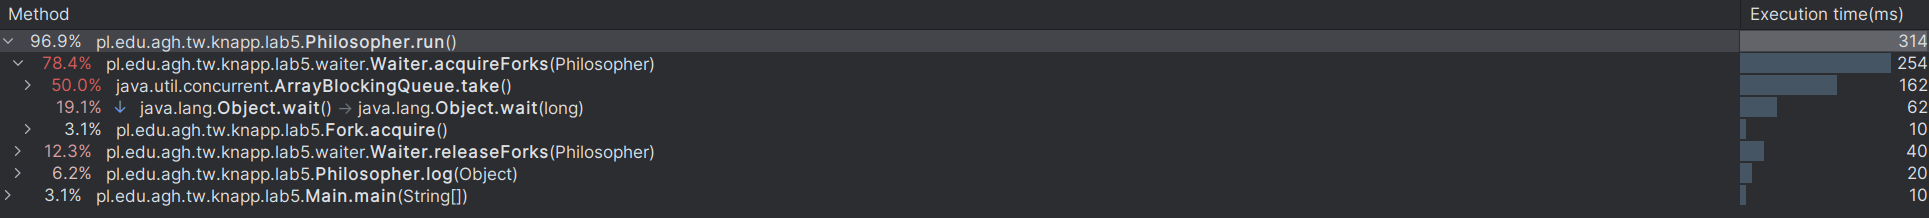
\includegraphics{profiler.png}
    \caption{profiler}
    \end{figure}
  \end{itemize}
\item
  \textbf{Autorskie rozwiązanie}, zgodnie z oczekiwaniami, jest najmniej
  wydajne - głównie z powodu wprowadzonych dodatkowych oczekiwań.
\item
  \textbf{Zakleszczenie (deadlock)} to sytuacja, w której procesy
  blokują się nawzajem z powodu zajęcia zasobów i żaden z procesów nie
  robi postępów, ponieważ czekają na zasób trzymany przez inny proces
\item
  W przypadku \textbf{zakleszczenia dynamicznego (livelock)}, z jednej
  strony stany zaangażowanych procesów ciągle się zmieniają. Z drugiej
  strony, procesy nadal są od siebie zależne i nigdy nie mogą zakończyć
  swoich zadań.
\item
  Podsumowując, zostały zaimplementowane 4 różne podejścia rozwiązujące
  problem pięciu filozofów, a mianowicie:

  \begin{enumerate}
  \def\labelenumi{\arabic{enumi}.}
  \tightlist
  \item
    \textbf{Naiwne podejście}, które może powodować zakleszczenia
  \item
    \textbf{Zaawansowane naiwne podejście} (\emph{autorskie
    rozwiązanie}), stosujące mechanizm oparty ma oczekiwaniu pewnej
    ilości czasu, która jest obliczana w oparciu o indeks filozofa oraz
    numer próby
  \item
    \textbf{Widelce podnoszone jednocześnie}: rozwiązanie to jest wolne
    od blokady, jednak w przypadku, gdy zawsze któryś z sąsiadów będzie
    zajęty jedzeniem, nastąpi zagłodzenie, gdyż oba widelce nigdy nie
    będą wolne
  \item
    \textbf{Rozwiązanie z lokajem}: jest to najbardziej zaawansowane
    rozwiązanie z wyżej wymienionych, polegające na tym, że zewnętrzny
    arbiter pilnuje, aby jednocześnie co najwyżej \(n-1\) filozofów
    konkurowało o widelce
  \end{enumerate}
\item
  \textbf{Ranking} zaimplementowanych rozwiązań \textbf{według
  wydajności}:

  \begin{enumerate}
  \def\labelenumi{\arabic{enumi}.}
  \tightlist
  \item
    Widelce podnoszone jednocześnie
  \item
    Rozwiązanie z lokajem
  \item
    Zaawansowane naiwne podejście
  \item
    Naiwne podejście (występuje zakleszczenie)
  \end{enumerate}
\end{itemize}

    \hypertarget{bibliografia}{%
\section{Bibliografia}\label{bibliografia}}

\begin{enumerate}
\def\labelenumi{\arabic{enumi}.}
\item
  Materiały do laboratorium, dr inż. Włodzimierz Funika:\\
  \url{https://home.agh.edu.pl/~funika/tw/lab5/}
\item
  Materiały do laboratorium, dr hab. inż. Bartosz Baliś\\
  \url{https://home.agh.edu.pl/~balis/dydakt/tw/lab8/tw-5fil.pdf}
\item
  Problem ucztujących filozofów - Wikipedia:\\
  \url{https://pl.wikipedia.org/wiki/Problem_ucztujących_filozofów}
\item
  Dining philosophers problem - Wikipedia:\\
  \url{https://en.wikipedia.org/wiki/Dining_philosophers_problem}
\item
  Deadlock, Livelock and Starvation - Baeldung:\\
  \url{https://www.baeldung.com/cs/deadlock-livelock-starvation}
\item
  \texttt{Object} - Java 17 Docs:\\
  \url{https://docs.oracle.com/en/java/javase/17/docs/api/java.base/java/lang/Object.html}
\item
  \texttt{ArrayBlockingQueue} - Java 17 Docs:\\
  \url{https://docs.oracle.com/en/java/javase/17/docs/api/java.base/java/util/concurrent/ArrayBlockingQueue.html}
\item
  \texttt{ConcurrentHashMap} - Java 17 Docs:\\
  \url{https://docs.oracle.com/en/java/javase/17/docs/api/java.base/java/util/concurrent/ConcurrentHashMap.html}
\item
  Carrier Sense Multiple Access (CSMA) - GeeksForGeeks:\\
  \url{https://www.geeksforgeeks.org/carrier-sense-multiple-access-csma/}
\end{enumerate}


    % Add a bibliography block to the postdoc
    
    
    
\end{document}
